\documentclass[10pt,a4paper]{article}
\usepackage[margin=19mm]{geometry}
\usepackage[utf8]{inputenc}
\usepackage{graphicx}\usepackage{booktabs}\usepackage{amsmath,amssymb}
\usepackage{parskip}\usepackage{array}\usepackage{tabularx}\usepackage{caption}
\usepackage{xcolor}
\usepackage[hidelinks]{hyperref}
\captionsetup{font=small,labelfont=bf}
\newcolumntype{Y}{>{\raggedright\arraybackslash}X}
\newcommand{\arm}[1]{\textbf{#1}}
\setlength{\tabcolsep}{4pt}

\title{\textbf{Real-Time Video Diffusion on One GPU:}\\[3pt]
\textbf{Where Self-Forcing Spends Its Time, and Forward-Only Control of When an Object Appears}\\[6pt]
\large A controlled study of Wan2.1-T2V-1.3B and its streaming distillation on an NVIDIA A100-40GB}
\author{Liad Mordechai\\
\small Computer Architecture final project - Prof.\ Avi Mendelson, Mr.\ Yaniv Nemcovsky \textperiodcentered{} Technion\\
\small Code, results and examples: \url{https://github.com/liadMor123/wan-realtime-control}}
\date{October 2026}

\begin{document}\maketitle

\begin{abstract}
Real-time text-to-video generation puts two demands on one GPU: every chunk of frames must be produced within a latency budget, and the result must follow the prompt, including \emph{when} things happen. This report studies both on the same model family, Wan2.1-T2V-1.3B and its chunk-wise autoregressive distillation Self-Forcing, on a single NVIDIA A100-SXM4-40GB.

\textbf{Part A (latency)} asks where a chunk-wise video diffusion transformer spends its time after CUDA graphs, and whether the persistent-megakernel result from memory-bound LLM decode transfers to this compute-bound regime. Using attribution by controlled intervention over thirteen jobs (J1-J13) with every threshold recorded before the job that tested it, we price three boundaries: kernel-launch boundaries are worth 3.11\,ms/pass after fusion (about 1\% of chunk time); an unanticipated RoPE-to-KV-cache materialization costs 19.7\,ms/pass, of which 10.7 was recovered byte-identically; and a wave-quantization tail in FlashAttention-2 (19.2\% of attention time, a 444-CTA grid on 108 SMs) is the only cost that clears the pre-registered 5\% gate. An off-the-shelf split-KV dispatch with an explicit split count recovers essentially all of that tail, so the persistent semaphore-scheduled kernel is reported as \emph{not justified} on this configuration. The integrated configuration cuts chunk-6 latency from 1{,}498 to 1{,}147\,ms ($-23.4\%$) with quality differences 4.6-7.0$\times$ smaller than a seed change. One Triton kernel built to fuse the split-KV combine into the output projection is numerically exact but 20\,ms/pass slower, with the register-budget mechanism identified by \texttt{ncu}.

\textbf{Part B (timing control)} asks whether TempoControl's gradient-based control of an object's appearance time, which costs about $2.6\times$ sampling time and about 110\,GB of memory, can be replaced by a forward-only edit. A per-frame logit bias on the object's text tokens in cross-attention ($+\beta$ on frames where the object should be visible, $-\gamma$ elsewhere, $\beta=\gamma=2$) raises TempoControl's official temporal-accuracy metric on Wan2.1 from 0.695 to 0.850 on all 80 single-object prompts (+15.5 points, 95\% CI [+11.1, +20.2]) against TempoControl's reported +19.7 (gains are compared, not absolute accuracies: our baseline scores 69.5\% to their 63.9\%, outside the pre-registered $\pm5$ band), on all 82 two-object pairs from 37.6\% to 47.2\% (+9.6, with a baseline that matches TempoControl's 37.5\%, so absolute accuracies are comparable there), and inside the real-time streaming model, where gradient-based control cannot run within the per-chunk latency budget or the memory of this GPU, from 0.617 to 0.875 (+25.8; replicated +24.2 at a second seed). It costs +0.8\% time over an fp32 explicit attention path (itself +6.5\%) and +1.58\% when carried inside Wan's own FlashAttention-2 kernel through eight padding head dimensions, with no extra memory, on a 40\,GB GPU. The method is essentially TS-Attn specialised to one object; the contribution is the measurement, including a pre-registered miss (VBench imaging quality $-0.043$) and a blinded substitute-object count that erases part of the gain against prompt switching.
\end{abstract}

\section{Introduction}

\subsection{Problem domain}
Diffusion transformers (DiTs) for text-to-video now run in real time by distilling a bidirectional model into a chunk-wise autoregressive one. Self-Forcing~\cite{selfforcing} distils Wan2.1-T2V-1.3B~\cite{wan} into a generator that produces a 5\,s, 81-frame video as seven chunks of three latent frames, each chunk denoised in four passes plus one clean-context pass that writes the chunk into a persistent KV cache. The streaming use case fixes the workload: batch size one, 4{,}680 tokens per chunk, thirty transformer blocks, attention K-length growing from 4{,}680 to 32{,}760 tokens within one video, all on a single GPU with a per-chunk latency budget. The same use case fixes the control problem: the user types a prompt with a timing instruction (``a car appears during the second second'') and the model must honour it without any extra denoising steps.

\subsection{The papers this project builds on}
\paragraph{Megakernels.} Hazy Research's persistent Llama-1B decode kernel~\cite{hazy} and MPK~\cite{mpk} report up to 1.7$\times$ over kernel-per-operator serving by replacing kernel boundaries with one persistent kernel whose work is ordered by semaphore counters. Both results are for memory-bound LLM decode on Hopper GPUs, where each kernel is small relative to its launch.

\paragraph{FlashAttention-2 and split-KV.} FlashAttention-2~\cite{fa2} parallelises attention over (batch, head, query-block) CTAs. At batch one with 12 heads and 37 query blocks the grid has 444 CTAs, which on 108 SMs is 4.11 waves launched as five. Flash-Decoding~\cite{flashdecoding} and Lean Attention~\cite{lean} split the K dimension across CTAs and combine partial results with a second kernel, which fills the last wave at the price of the combine.

\paragraph{TempoControl.} TempoControl~\cite{tempocontrol} controls \emph{when} an object appears in Wan2.1-T2V-1.3B by running gradient descent on the latent during sampling, with a loss on the cross-attention maps of the object's tokens, and defines a benchmark (80 single-object prompts, 82 two-object pairs) with an official metric: YOLOv10x~\cite{yolov10} detects the object in 20 evenly spaced frames and a frame scores when detection matches a per-frame visibility mask. It raises single-object accuracy from 63.9\% to 83.6\% (+19.7 points) and two-object accuracy from 37.5\% to 53.2\%. Its reference implementation requires about $2.6\times$ the sampling time and about 110\,GB of GPU memory, against 13.8\,GB for plain sampling in our runs, which rules it out on a 40\,GB A100 and in a streaming setting, where backpropagating through each chunk would not fit the per-chunk latency budget.

\paragraph{Training-free attention control.} DenseDiffusion~\cite{densediffusion} modulates attention logits by $\pm$ terms for spatial layout. TS-Attn~\cite{tsattn} adds a positive bias to a target's text tokens on its frames and a negative bias elsewhere, early in sampling, on Wan2.1-14B and Wan2.2, for multi-event videos. Prompt Relay~\cite{promptrelay}, TALC~\cite{talc} and Peekaboo~\cite{peekaboo} split captions per frame or mask text keys out with $-\infty$. For streaming models, LongLive~\cite{longlive} and Rolling Forcing~\cite{rollingforcing} switch prompts at chunk boundaries, differing in whether the self-attention cache is rebuilt after the switch.

\subsection{Drawbacks addressed}
Four gaps motivated Part A: no ablation that separates \emph{scheduling} from ordinary kernel fusion; no evidence on a compute-bound DiT; no Ampere data; and no per-position latency reporting for a workload whose cost grows within a single generation. The last turned out to matter most: chunk time rises from 804 to 1{,}498\,ms over one seven-chunk video, so any single ``chunk latency'' number is meaningless without its position.

Part B addresses TempoControl's cost: its gradient optimisation needs memory a 40\,GB GPU does not have and time a real-time system does not have. The question is whether a forward-only edit of the model's text cross-attention, with no gradients, no extra steps, unchanged weights and the prompt text left as it is, recovers a useful fraction of the gain on TempoControl's own benchmark and metric, at what cost, and whether it extends to the streaming model where gradient methods cannot run. A secondary question is what such an edit costs in video quality and in failure modes the official metric does not see.

\subsection{Contributions}
(1) A priced decomposition of Self-Forcing's chunk time on A100 with every threshold pre-registered, and the verdict that a persistent megakernel is not justified there because an off-the-shelf split-KV dispatch already recovers the one cost that clears the gate; a 23.4\% chunk-6 latency reduction from conventional fixes; and a measured negative result for a fused split-KV-merge GEMM kernel with its mechanism. (2) The measurement that a forward-only per-frame cross-attention bias recovers 79\% of TempoControl's single-object gain on its full benchmark (62-86\% across seeds on the held-out set) and 61\% of its two-object gain, at under 2\% extra time and no extra memory, carried inside an unmodified FlashAttention-2 kernel, and gives +25.8 points inside the real-time streaming model; together with prompt-switching baselines, a blinded failure-mode count, VBench quality, and three mechanistic findings (padding tokens absorb about 92\% of cross-attention; absolute share targeting fails because it flattens spatial attention; too strong a bias destroys the video when the ``off'' window is the start).

\section{Methods}

\subsection{Part A: attribution by controlled intervention}
Every number in Part A is a difference between two measured configurations that differ in exactly one component, never a roofline subtraction. Chunk time is modelled per position as $t(K)=a+bK$ with $K$ the attention K-length; the fit has $R^2\ge0.9996$ in every seven-position mode, so the K-independent intercept $a$ and the slope $b$ can be attributed separately.

\paragraph{The capture-enabling patch.} The reference implementation cannot be captured into a CUDA graph, not because of dynamic shapes but because of five host-device synchronisations on the per-pass path, including a \texttt{.item()} on the KV-cache index. Removing them is host-side plumbing whose acceptance test is byte-identical video output on all five prompts, which passed. The patch is a prerequisite, not a result.

\paragraph{The census, the tails, the arm, the gate.} J5 classified all 1{,}319 CUDA kernel launches per pass and reconciled their sum with the independent timing fit (criterion 3\%). J6 measured wave-quantization tails with \texttt{ncu} and, independently, with a head-count sweep. The gate for building a persistent kernel on a segment $S$ was frozen before J6:
\[
\text{gate}_S(\text{pos}) = \frac{100\cdot(r_S\cdot 5)}{\text{chunk time}_{\text{graphed-compiled}}(\text{pos})},\qquad \text{threshold } 5\%,
\]
with $r_S$ the recoverable tail per pass and five passes per chunk. J7 then measured the conventional arm, \texttt{flash\_attn\_with\_kvcache} with an explicit \texttt{num\_splits}, and the persistent-kernel build threshold was a residual tail of 4\% of chunk time at position 6, frozen before the residual was computed. J10 derived a position-dependent split rule from measured quantities.

\paragraph{The one kernel built (J13).} The split-KV arm pays a K-independent 5.35\,ms/pass for FA2's combine pass. J13 asked whether folding that merge into the prologue of the output-projection GEMM removes it. A 4-file source patch to FlashAttention-2 v2.8.3 adds a \texttt{return\_partials} flag (combine skipped, fp32 per-split outputs and log-sum-exps returned); a Triton kernel merges one head's partials per K-step with weights $\exp(\text{lse}_s-\text{LSE})$, casts to bf16 at the same point as FA2's combine, and feeds the tile to the GEMM, bias in the epilogue. Two forecasts were recorded before any run.

\subsection{Part B: forward-only per-frame cross-attention bias}
In every one of Wan's 30 blocks each video token attends to the same 512 text tokens from the umT5 encoder. The video is 21 latent frames $\times$ 30 $\times$ 52 patches $=32{,}760$ query tokens; all of them see the same text keys, and the text encoder has no notion of frames. Boosting attention to the timing words (``during the second second'') therefore pushes every frame identically and cannot make frame 5 differ from frame 15. Timing information has to enter \emph{per frame}. Every arm has three parts: a per-frame visibility mask $m\in\{0,1\}^{21}$ (Wan's VAE maps latent frame 0 to output frame 0 and latent frame $j\ge1$ to output frames $4j-3\ldots4j$; a parser for free-form phrases reproduces all 80 benchmark masks exactly), the object's token positions $O$ in the 512-slot context (sentencepiece pieces found by character offsets; they match TempoControl's own lookup on all 80 prompts), and a per-frame edit of the cross-attention logits for queries $q$ in frame $f(q)$.

Cross-attention computes $a_{q,i}=\mathrm{softmax}_i(\ell_{q,i})$ with $\ell_{q,i}=q\cdot k_i/\sqrt d$. With $T$ the timing phrase's positions, the arms are:
\begin{center}\small
\begin{tabularx}{\textwidth}{lYl}\toprule
Arm & Edit & Parameters tested\\\midrule
\arm{B0} & none (plain Wan2.1-1.3B on the benchmark prompt) & - \\
\arm{U} (control) & $\ell_{q,i}\mathrel{+}=\beta$ for $i\in T$, on every frame & $\beta=2$\\
\arm{L} (logit bias) & $\ell_{q,i}\mathrel{+}=\beta$ if $m_{f(q)}=1$, $-\gamma$ if $m_{f(q)}=0$, for $i\in O$ & $(\beta,\gamma)=(2,2),(4,4)$\\
\arm{S} (share targeting) & per query, shift $\ell_O$ by $\delta=\mathrm{logit}(s^*)-(\mathrm{lse}\,\ell_O-\mathrm{lse}\,\ell_{\neg O})$ so that $\sum_{i\in O}a_{q,i}=s^*$, with $s^*=s_{hi}$ on ``on'' frames and $s_{lo}$ on ``off'' frames & $(s_{hi},s_{lo})=(0.01,10^{-4}),(0.05,10^{-4})$\\
\arm{P} (prompt split) & $\ell_{q,i}=-\infty$ for $i\in O$ on frames with $m=0$ & - \\
\arm{Schedule} & apply the best arm only in denoising steps $<k$ & $k=10$ of 50\\
\bottomrule\end{tabularx}
\end{center}
The edit is applied only in the conditional branch of classifier-free guidance (the unconditional branch sees Wan's negative prompt, which contains no object tokens), in all 30 blocks and all 12 heads. Padding is attended: Wan passes no length mask, so the 483 padding slots are part of every softmax, exactly as the model sees them. \arm{L} multiplies every query's odds for the object by the same factor $e^{\beta}$ and so preserves the spatial pattern of attention; \arm{S} forces all 1{,}560 queries of a frame to the same share and so destroys it. This difference turned out to decide the outcome. For two objects (\arm{L}, $K=2$), each object's bias goes on its own token set with its own mask, so the static object gets $+2$ on every frame.

\paragraph{Production path (fa2kv).} We call this path fa2kv (FlashAttention-2 with an additive key-side bias). \arm{L}'s bias is rank-1 per frame, $b(f)\cdot\mathbb{1}[i\in O]$, so it can be carried inside an unmodified FlashAttention-2 call by augmenting the head dimension from 128 to 136: $q$ carries $b(f)$ in three of the eight padding dims (the rest are zero), the object keys carry bf16 constants $c_0+c_1+c_2=1/\mathrm{fp32}(128^{-1/2})$ in those dims (so that the dot product, after FA2's \texttt{softmax\_scale}$=128^{-1/2}$, adds exactly $b(f)$), the other keys carry zeros, and $v$ is zero-padded. FA2 2.8.3 runs its hdim-192 kernel for $d=136$. With a zero table the output is bitwise equal to Wan's own flash call, so the same code path serves as \arm{B0}.

\paragraph{Streaming (Self-Forcing).} Self-Forcing has no CFG and generates seven chunks of three latent frames. \arm{L} is a static $21\times512$ table indexed by each chunk's frame offset (\texttt{current\_start}), applied in all four denoising passes and the clean-context pass of every chunk, through the fa2kv path. The obvious streaming alternative is \emph{prompt switching}: generate the pre-onset chunks from ``An empty scene.'' (the first sentence of every benchmark prompt, verbatim) and switch to the full prompt at the onset chunk $\lfloor\text{first\_on}/3\rfloor$. Three variants were run on the same path: \arm{PS-RF} (Rolling-Forcing-style: re-cache only the cross-attention K/V, keep the self-attention cache), \arm{PS-LongLive-style} (rebuild both caches, ported from LongLive~v1's \texttt{\_recache\_after\_switch}), and \arm{PS-RF+L}.

\section{Implementation and experiments}

\subsection{Hardware and software}
All GPU work ran on NVIDIA A100-SXM4-40GB nodes (108 SMs, MIG disabled, driver 595.71.05) of the Technion Athena Slurm cluster; no larger-memory GPU was used anywhere. Part A: PyTorch 2.7.1+cu126, Triton 3.3.1, flash-attn 2.8.3.post1, Python 3.11, Self-Forcing pinned at \texttt{33593df3}, measured HBM bandwidth 1{,}380\,GB/s. Part B: Wan2.1 at \texttt{9737cba} (unmodified; cross-attention patched at runtime), TempoControl at \texttt{ac28c443} (data and metric only), Self-Forcing cloned from Part A's \texttt{capture-enable} branch onto branch \texttt{tempo-L} @ \texttt{d3dc62f}; metric environment YOLOv10 fork @ \texttt{453c6e38} with \texttt{huggingface\_hub} 0.23.4, VBench 0.1.5, OpenCLIP ViT-L-14-quickgelu. Compute-node scratch is wiped between jobs, so every job stages weights to \texttt{\$TMPDIR} and copies back reduced results only.

\subsection{What is upstream and what is ours}
Upstream and unmodified: Wan2.1, Self-Forcing, FlashAttention-2, Inductor, TempoControl's benchmark CSVs and \texttt{temporal\_accuracy.py}, YOLOv10x, VBench. Ours, Part A: a 16-commit patch series to Self-Forcing (9 commits of byte-identical capture-enabling plumbing, 3 of byte-identical cache-write fusion, 1 flag-gated split-KV API swap, 1 optional position-dependent dispatch, 2 for the J13 kernel), the 4-file \texttt{return\_partials} patch to FlashAttention-2, the Triton fused-merge kernel, the timing harness, census and tail scripts, and all analysis and plotting. Ours, Part B: the explicit cross-attention path and all five arms (\texttt{cross\_attention\_arms.py} in \texttt{src/tempo\_ctrl/}), the fa2kv head-augmentation (\texttt{fused\_attention.py}), the sampling loop that mirrors Wan's \texttt{generate} (\texttt{sampler.py}), the mask parser and token lookup (\texttt{masks.py}, \texttt{tokens.py}), the \texttt{tempo\_bias} hook and prompt-switching code in the Self-Forcing clone, the Phase-0 test suite, generation, scoring, bootstrap and figure scripts, and 62 CPU unit tests. No metric script was modified.

\subsection{Part A: experiments J1-J13}
Thirteen jobs were run; J11 and J12 were diagnostic reruns that produced no headline number and are omitted from the appendix.
Five prompts, fixed seeds, seven chunk positions; the first video is warm-up and excluded; the statistic is the median per position, with spread $100\cdot(\max-\min)/\text{median}$ (0.1-0.6\% at chunk 6, at most 1.04\% anywhere). Timing definitions were frozen in J2: a chunk boundary is a synchronised host timestamp after the fifth pass; per-pass times are CUDA events read only after the whole generation so measurement does not serialise host and device; the VAE decode is a separate stage. Modes: \emph{eager-original}; \emph{final} (sync sites removed, cache-write fusion, Inductor fusion in \texttt{max-autotune} mode, manual CUDA graphs over compiled kernels, split-KV with $s=4$); and leave-one-out variants. Median per position is the headline statistic because the cost grows within a video and run-to-run spread is below 1\%; profiler-attached rows are attribution data and are never quoted as latency. No model was trained in either part of this project. Numerics use three tiers: bitwise identity where identity is expected; single-pass agreement against an fp32 eager reference within $2\times$ the bf16 band measured in the same job; and distributional quality (CLIP prompt similarity, CLIP temporal consistency, LPIPS over ten prompts), descriptive only. Per-frame PSNR against an eager reference was retired in J3 because a 35-pass autoregressive sampler amplifies bf16 reduction-order changes into a different-but-valid sample (minimum 14.4\,dB against a 40\,dB floor that was not loosened).

Harness constraints discovered and worked around: manual CUDA graphs and Inductor cannot share a process; graph modes cannot be interleaved with non-graph modes; \texttt{ncu -c 1} ignores \texttt{cudaProfilerStart}, so \texttt{--profile-from-start off} is required (caught because FA2 reported identical durations at two positions whose cost must differ by $1.75\times$). An independent validation re-measured eager-original and final from a clean clone plus the patch series: eager-original reproduces within 0.4\% at every position and the chunk-6 reduction re-measures at 23.7\%.

\subsection{Part B: experiments}
\paragraph{Benchmark and metric.} TempoControl's \texttt{one\_object.csv}: 80 prompts of the form \emph{``An empty scene. Suddenly, during the $\langle$second $|$ third $|$ fourth $|$ last$\rangle$ second of the video, a $\langle$COCO object$\rangle$ appears out of nowhere, drawing all attention.''}, 20 per timing, and \texttt{two\_objects.csv}: 82 pairs with a static object present throughout and a temporal object appearing from latent frame 10 (17 pairs are capped by the metric whatever the method does). Throughout, frames with $m=0$ are called \emph{absent frames} and frames with $m=1$ \emph{present frames}; ``absent ok'' is the fraction of absent frames in which the object class is not detected, ``present ok'' the fraction of present frames in which it is. Metric: the official \texttt{temporal\_accuracy.py}, unmodified, YOLOv10x on 20 evenly spaced frames; a video's accuracy is the fraction of frames whose detection matches the mask. Protocol (TempoControl's): $832\times480$, 81 frames, UniPC~\cite{unipc} sampler, 50 steps, shift 3, CFG 6, Wan's default negative prompt; seed 42 is TempoControl's seed, 43 the replication seed. The official metric is used because it is the yardstick TempoControl's own numbers are stated in; it only checks class detection per frame, so secondary metrics guard what it does not see: CLIP prompt similarity (ViT-L-14-quickgelu) for prompt adherence, VBench imaging quality (MUSIQ-SPAQ) and subject consistency (DINO) for perceptual cost, $4\times4$ contact sheets, and a blinded count of \emph{substitute objects} (another object rendered on ``off'' frames and morphed into the target at onset), judged on 400 shuffled sheets in batches by separate judges under a rule fixed before looking, verdicts committed before unblinding.

\paragraph{Prompt sets and pre-registration.} Because the benchmark file is sorted by timing, prompt sets were stratified: a pilot of 8 prompts (ids 0, 1, 20, 21, 40, 41, 60, 61) for choosing arms; 20 held-out prompts (ids 2-6, 22-26, 42-46, 62-66) never used for any choice; the remaining 52 added in step 4 for the full benchmark; the 72 \emph{non-pilot} prompts are the 80 minus the 8 pilot ids. Arms, parameters, prompt sets, predictions and thresholds were frozen in \texttt{experiment\_spec.md} and committed to git before the runs they affect; every decision carries its date and commit. Comparisons are paired per prompt: mean difference, 95\% bootstrap CI (10{,}000 resamples), better/worse counts with a sign test.

\paragraph{Phase 0: tests of the measurement.} Before any comparison: our sampling loop against Wan's own \texttt{generate} (byte-identical video); the explicit attention path with a zero edit against explicit \arm{B0} (byte-identical, so arms differ only in the edit); explicit versus flash attention against an fp64 reference at 9 probes (explicit at least as accurate everywhere; full videos nevertheless differ, PSNR 22\,dB, because rounding-order differences compound over 50 steps, which is why \arm{B0} must run on the same path as the arms); \arm{S} reaches its target share to $3\cdot10^{-15}$ in fp64; \arm{P} gives object share exactly 0 on off frames; metric preflight on synthetic videos (exact); tokenizer and mask tests. An attention diagnostic on one \arm{B0} video showed that the 483 padding slots take about 92\% of all cross-attention, the object token about 0.1\%, and the timing phrase 0.6-1.2\%. This fixed the scale of the edits ($\beta=2$ multiplies the object's odds by $e^2\approx7.4$) and forced a re-parametrisation of \arm{S} before the pilot, since the plan's original $s_{lo}$ would have \emph{raised} the object's attention 20-40$\times$ on off frames. Environment faults found and fixed in this phase included a \texttt{huggingface\_hub} version under which the YOLOv10 loader silently trained a fresh model that detects nothing; the metric script now fails loudly if this recurs.

\paragraph{Steps.} Phase 1, pilot (56 videos, 7 arms $\times$ 8 prompts, plus 8 for the schedule variant); Phase 2, held-out (B0 at seeds 42 and 43, L(2,2), L(4,4), L(2,2) $k{<}10$ $\times$ 20 prompts, plus seed-43 replication of the two L(2,2) arms); step 2, fa2kv production path with a 9-probe numerical test and a matched-baseline accuracy check against Wan's unmodified flash path; steps 3 and 3b, \arm{L} inside Self-Forcing on 20 and then all 80 prompts at two seeds, with latency in Part A's per-position protocol (\emph{final} mode); steps 3b-2 and 3c, prompt-switching baselines on all 80 prompts with six machinery gates (M0-M5, e.g.\ an identity switch at chunk 3 must equal plain generation); step 4, the full 80-prompt Wan benchmark; steps 5a/5b, two objects on 20 and then all 82 pairs; step 6, VBench. Total: 13.0 GPU-hours for Part 1 and 22.8 for Part 2, all A100.

\section{Results and discussion}

\subsection{Part A: where the time goes}
\paragraph{Decomposition and census (Fig.~\ref{fig:a1}, \ref{fig:a2}).} Of the 136.6\,ms/pass K-independent cost of the unpatched eager baseline, host-device sync sites account for 9.60\,ms/pass, Inductor fusion and kernel selection for 26.81, and launch boundaries after fusion for 3.11, leaving 97.06\,ms/pass. Fusion is worth about five times the launch-boundary saving measured over eager kernels (26.81 vs 4.99\,ms/pass) and about nine times the saving after fusion. Of 96.2\,ms/pass of K-independent work, GEMM arithmetic at peak is 37.6, GEMM inefficiency 20.7, KV-cache writes and device-to-device copies 19.7, elementwise and norm 14.8, cross-attention 3.5: only 39\% is tensor-core arithmetic at peak, and the cache-write bucket runs at 15.8$\times$ the bandwidth floor, a data-movement cost the arithmetic model does not contain.

\paragraph{Tails and the conventional arm (Fig.~\ref{fig:a3}, \ref{fig:a4}).} FA2 self-attention has a 19.2\% tail at position 6 at 55.8\% SM throughput and 3.1\% DRAM. A head-count sweep confirms the mechanism independently: kernel time is flat within each step and jumps where $\lceil 37H/108\rceil$ increments, implying an effective wave of 108 CTAs, and the implied waste at $H=12$ is 19.4\% against 19.2\% measured. The FFN down-GEMM, the segment originally proposed for a persistent kernel, has a tail of only 7.7\% and fails the 5\% gate; only the attention tail (9.5-12.1\% of chunk time) passes. Self-attention is the largest single consumer in any case: 165.6 of 262.6\,ms of device time in a chunk-6 pass, 63\%, at 170.7\,TFLOP/s (55\% of the A100's dense bf16 peak) with 3.1\% DRAM throughput. \texttt{flash\_attn\_with\_kvcache} with \texttt{num\_splits}=4 recovers 19.53\% at position 6 and 19.63\% at position 3, flattening the staircase to a 3.0\% spread. Left to its heuristic, FA2 picks about one split and recovers only 3.05\% of attention time: the split count must be set explicitly. The residual tail after the arm is not measurable (clipped at 0) against the 4\% build threshold, so the persistent kernel is not justified on this configuration. One qualification belongs next to the verdict: measured at chunk level rather than at the attention kernel, 8.83\,ms/pass (3.36\% at position 6, 4.36\% at position 3) still goes unrecovered, and that quantity is consistent with the split-KV arm's own K-independent overhead (combine pass and partial buffers), not with residual quantization. A kernel that fused the combine away would attack that smaller target; J13 below is the attempt.

\begin{table}[htbp]\centering\small
\caption{Part A master table: median chunk time (ms) over five videos, with the per-position fit $t=a+bK$ ($a$ in ms, $b$ in ms per 1{,}000 K-tokens). The two J13 rows are from their own job and compare within it.}
\label{tab:master}
\begin{tabular}{lrrrrrr}\toprule
mode & pos 0 & pos 3 & pos 6 & $a$ & $b$ & $R^2$\\\midrule
eager-original & 803.7 & 1146.8 & 1498.3 & 682.75 & 24.861 & 0.99989\\
\textbf{final} & \textbf{559.0} & \textbf{855.9} & \textbf{1147.0} & 464.22 & 20.937 & 0.99980\\
final $-$ graphs & 573.4 & 864.9 & 1155.0 & 476.70 & 20.780 & 0.99987\\
final $-$ cache-write fusion & 607.6 & 902.3 & 1192.9 & 512.75 & 20.828 & 0.99981\\
final $-$ split-KV & 553.8 & 904.4 & 1254.8 & 437.48 & 24.948 & 1.00000\\
final $-$ Inductor & 678.3 & 955.7 & 1241.8 & 582.22 & 20.115 & 0.99975\\
final\_rule (J10, position-dependent split) & 553.0 & 856.3 & 1161.7 & 456.63 & 21.432 & 0.99964\\
final (J13 companion run) & 566.7 & 868.0 & 1159.7 & 471.28 & 21.121 & 0.99977\\
final + fused merge (J13) & 668.5 & 969.2 & 1263.4 & 571.54 & 21.215 & 0.99979\\
\bottomrule\end{tabular}
\end{table}

\paragraph{The integrated result (Table~\ref{tab:master}, Fig.~\ref{fig:a5}, \ref{fig:a6}).} \emph{final} reduces chunk-6 time from 1{,}498.3 to 1{,}147.0\,ms ($-23.4\%$) and chunk 3 by 25.4\%, intercept 682.75 $\to$ 464.22 and slope 24.86 $\to$ 20.94. Leave-one-out heights at chunk 6: split-KV 107.9\,ms, Inductor fusion 94.9, sync sites 48.0, cache-write fusion 45.9, graphs 8.0; the bars sum to 304.6 against a measured 351.4, a $-13.3\%$ interaction, stated rather than hidden. \emph{final $-$ split-KV} reproduces the eager slope within 0.35\%, so split-KV is the only component with a large slope effect; its intercept gap to \emph{final}, 5.35\,ms/pass, is the K-independent cost of the combine pass and partial buffers. The J10 position-dependent rule predicts attention time to 1.54\% mean absolute error yet loses to a fixed $s=4$ by 1.12\%, because across the splits it discriminates between measured time varies by only 0.9-2.8\%, the same order as the model's error.

\paragraph{Quality (Fig.~\ref{fig:a8}).} Over ten prompts, changing the random seed moves CLIP prompt similarity 4.6$\times$, CLIP temporal consistency 6.1$\times$ and LPIPS 7.0$\times$ further than the entire optimisation stack does. Descriptive only.

\paragraph{The fused split-KV merge (J13): a measured negative result.} Correctness held everywhere: at all seven positions and both split counts the fused kernel's error against an fp32 merge of the same partials equals the PyTorch bf16 path's to three digits, and in situ its single-pass error is identical to \emph{final}'s. Cost: at $s=4$, position 6, the fused kernel takes 1.10\,ms per layer against 0.17\,ms for the cuBLAS out-projection plus 0.21\,ms for the combine it replaces; integrated, \emph{final + fused merge} is slower than \emph{final} by a K-independent 100-104\,ms per chunk (+20.05\,ms/pass; +18.0\% at chunk 0, +8.9\% at chunk 6). \texttt{ncu} names the mechanism: 255 registers per thread cap occupancy at one 256-thread block per SM and spill about 50\,MB per launch; the fp32$\times$4 partials are re-read once per N-block (2.67\,GB of L2 traffic against 0.32\,GB for the GEMM); with one pipeline stage the merge serialises before the MMA and the tensor pipe is active 9.0\% of the time against 80.7\% in the GEMM it replaces. DRAM bandwidth and wave quantization are not the mechanism. The generalisation: a merge prologue pays only if its inputs are read once per row block, which places it in a full-N/small-M tiling or in the attention kernel's epilogue, not in an N-tiled projection GEMM.

\paragraph{What transfers from the megakernel literature.} The megakernel result removes barrier and launch overhead in a memory-bound decode where each kernel is small relative to its launch. Here, after ordinary fusion, that overhead is about 1\% of chunk time. What dominates is grid quantization inside one large kernel, a scheduling problem, but one an off-the-shelf split-KV dispatch already solves. On this configuration the machine was left idle by tail waves inside one kernel, not by kernel boundaries. At the frame-level regime a streaming system might run (one latent frame per chunk, Fig.~\ref{fig:a7}) the grid is 156 CTAs, 1.44 waves, with 27.8\% quantization waste by grid arithmetic and 22\% higher K-independent cost per token; that regime was not measured and is where a future kernel would have to beat the split-KV integration as its baseline.

\subsection{Part B: controlling when the object appears}

\paragraph{Pilot (8 prompts, seed 42).} \arm{B0} fails the way TempoControl describes: the object is usually on screen from the start, so absent frames are correct only 47\% of the time. \arm{L}(2,2) fixes exactly that (absent-frame accuracy 0.47 $\to$ 0.93, present frames unchanged; mean accuracy 0.688 $\to$ 0.919, 7 prompts better / 0 worse). \arm{U} changes nothing (+0.012, 3/3), as predicted: a frame-independent boost cannot move timing. \arm{P} can only remove the object, never strengthen it (0.781). \arm{S} never lets the object form (0.59): forcing every query of a frame to the same share erases the spatial contrast that localises the object, and the contact sheets show abstract gray shapes. By the pre-committed rule, \arm{L}(2,2) and \arm{L}(4,4) went to the held-out phase, with the $k{<}10$ schedule.

\begin{table}[htbp]\centering\small
\caption{Held-out results on Wan2.1 (20 prompts never used for any choice). $\Delta$ is the paired mean difference in accuracy against \arm{B0} at the same seed, with 95\% bootstrap CI and better/worse counts (sign test $p$). Recorded peak memory is 13.84\,GB for every run (see Appendix~B).}
\label{tab:heldout}
\resizebox{\textwidth}{!}{\begin{tabular}{llrlrrrr}\toprule
seed & run & acc. & $\Delta$ vs B0 [CI] & better/worse ($p$) & absent ok & present ok & time vs B0\\\midrule
42 & B0 (reference) & 0.705 & - & - & 0.64 & 0.77 & - \\
43 vs 42 & B0 seed 43 (seed control) & 0.772 & +0.068 [$-$0.037, +0.170] & 11/6 (0.33) & 0.71 & 0.83 & -\\
42 & \arm{L}(2,2) & \textbf{0.875} & \textbf{+0.170 [+0.092, +0.255]} & 12/1 (0.003) & 0.80 & 0.95 & +0.8\%\\
42 & \arm{L}(2,2), steps $<10$ & 0.872 & +0.168 [+0.087, +0.255] & 11/1 (0.006) & 0.79 & 0.96 & +0.1\%\\
42 & \arm{L}(4,4) & 0.795 & +0.090 [$-$0.075, +0.237] & 14/5 (0.064) & 1.00 & 0.59 & +0.8\%\\\midrule
43 & B0 & 0.772 & - & - & 0.71 & 0.83 & - \\
43 & \arm{L}(2,2) & \textbf{0.895} & \textbf{+0.123 [+0.030, +0.220]} & 13/1 (0.002) & 0.90 & 0.90 & - \\
43 & \arm{L}(2,2), steps $<10$ & 0.855 & +0.082 [+0.005, +0.170] & 12/2 (0.013) & 0.88 & 0.83 & - \\\midrule
pooled & \arm{L}(2,2), 40 pairs & & +0.146 [+0.084, +0.210] & 25/2 & & &\\
\bottomrule\end{tabular}}
\end{table}

\paragraph{Held-out (Table~\ref{tab:heldout}, Fig.~\ref{fig:b1}).} \arm{L}(2,2) raises accuracy from 0.705 to 0.875 (+17.0 points), beats the seed-to-seed control as well (+0.102, $p=0.002$), and replicates at the second seed (+12.3). A single video's accuracy moves by about 0.18 just from changing the seed (B0 s43 $-$ B0 s42: mean $|\Delta|$ 0.177, sd 0.241), so the evidence rests on paired counts and CIs, not on individual prompts. \arm{L} helps most where \arm{B0} is worst, the late timings (4th and last second: 0.58/0.62 $\to$ 0.82/0.79) and does not hurt the easy ones. \arm{L}(4,4) breaks when the ``off'' window is the start of the video: on 4 of the 5 ``second second'' prompts the video collapses into stripe texture (group mean 0.35), while on later timings it is the most accurate run (0.92-0.97). So the right strength depends on the timing and $\beta=\gamma=2$ is the robust setting. Editing only the first 10 of 50 steps keeps 85\% of the gain pooled over seeds (99\% at seed 42, 67\% at 43), consistent with layout being decided early but not fully stable.

\begin{table}[htbp]\centering\small
\caption{Full benchmarks. Wan2.1 single object on the explicit path (seed 42); Self-Forcing single object on the fa2kv path (two seeds; \arm{B0} is bitwise identical to unmodified Self-Forcing); Wan2.1 two objects. TempoControl's numbers are quoted from its paper.}
\label{tab:full}
\resizebox{\textwidth}{!}{\begin{tabular}{llrrlrll}\toprule
model & set & B0 & \arm{L} & $\Delta$ pts [95\% CI] & better/worse & absent B0$\to$L & present B0$\to$L\\\midrule
Wan2.1 & all 80 prompts & 0.695 & \textbf{0.850} & \textbf{+15.5 [+11.1, +20.2]} & 56/7 & 0.59 $\to$ 0.88 & 0.80 $\to$ 0.82\\
Wan2.1 & 72 non-pilot & 0.696 & 0.842 & +14.7 [+9.9, +19.6] & 49/7 & 0.61 $\to$ 0.87 & 0.78 $\to$ 0.82\\
\emph{TempoControl (paper)} & all 80 & 0.639 & 0.836 & +19.7 & & &\\\midrule
Self-Forcing, s42 & all 80 & 0.617 & \textbf{0.875} & \textbf{+25.8 [+20.8, +30.9]} & 66/5 & 0.45 $\to$ 0.95 & 0.78 $\to$ 0.80\\
Self-Forcing, s43 & all 80 & 0.601 & \textbf{0.843} & \textbf{+24.2 [+19.1, +29.5]} & 64/9 & 0.38 $\to$ 0.88 & 0.82 $\to$ 0.81\\
Self-Forcing, s42 & 72 non-pilot & 0.631 & 0.867 & +23.7 [+18.7, +28.7] & 58/5 & 0.49 $\to$ 0.95 & 0.78 $\to$ 0.79\\\midrule
Wan2.1, $K{=}2$ & all 82 pairs & 0.376 & \textbf{0.472} & \textbf{+9.6 [+4.2, +15.0]} & 40/16 & 0.49 $\to$ 0.61 & 0.27 $\to$ 0.35\\
Wan2.1, $K{=}2$ & 65 scorable pairs & 0.450 & 0.566 & +11.6 [+5.2, +18.2] & 38/15 & & \\
\emph{TempoControl (paper)} & all 82 pairs & 0.375 & 0.532 & +15.7 & & &\\
\bottomrule\end{tabular}}
\end{table}

\paragraph{The full Wan benchmark (Table~\ref{tab:full}, Fig.~\ref{fig:b2}).} On all 80 prompts \arm{L} gives +15.5 points (56 better / 7 worse) against TempoControl's reported +19.7: 79\% of the gradient-based gain. The pre-registered calibration gate was missed: our \arm{B0} scores 69.5\% against TempoControl's 63.9\%, outside the $\pm5$ band, so the absolute numbers are not comparable and only gains are. By timing, the paired gain is +8.5 / +4.5 / +18.0 / +31.0 points for the 2nd / 3rd / 4th / last second.

\paragraph{Two objects.} On the first 20 scorable pairs \arm{L} with $K=2$ gives +20.2 points; on all 82 pairs it gives +9.6 (37.6\% $\to$ 47.2\%). Here the baselines agree (37.6\% vs TempoControl's 37.5\%), so the absolute comparison holds: 47.2\% against their 53.2\%, 61\% of their gain. The 20-pair estimate was optimistic: the other 62 pairs gain +6.1 [+0.2, +11.9], mostly by keeping the temporal object out of the off frames; getting both objects onto the on frames remains hard (0.22 $\to$ 0.24 on those pairs).

\paragraph{Streaming (Table~\ref{tab:full}, Fig.~\ref{fig:b3}).} Inside Self-Forcing, where TempoControl cannot run within the latency budget, \arm{L} gives +25.8 and +24.2 points at two seeds on all 80 prompts, with absent-frame accuracy 0.45 $\to$ 0.95 and present frames flat. The gain grows with lateness (last second +41/+44 points, second second +12/+6). A 20-prompt drop in present-frame accuracy (0.91 $\to$ 0.81) did not generalise to 80 prompts. Latency in Part A's protocol: +1.58\% on the mean over positions (numerically the same figure as the fa2kv cost on Wan below; a coincidence of two separate measurements), +2.2\% and +2.1\% at positions 0-1 (11-14\,ms per chunk), so the pre-registered 2\% cost bound was met on the mean and missed at the first two positions. Our literature passes found no prior forward-only, training-free per-frame timing control inside a streaming video model.

\begin{table}[htbp]\centering\small
\caption{Prompt-switching baselines in Self-Forcing, all 80 prompts, seed 42, same fa2kv path. The blinded substitute-object count treats every absent frame of a counted video as failed.}
\label{tab:ps}
\resizebox{\textwidth}{!}{\begin{tabular}{lrlrrrrr}\toprule
arm & acc. & $\Delta$ vs \arm{L} pts [CI] & absent ok & present ok & CLIP $\Delta$ vs B0 & substitutes /80 & absent, corrected\\\midrule
B0 & 0.617 & - & 0.45 & 0.78 & - & 6 & 0.405\\
\arm{L} & 0.875 & - & 0.95 & 0.80 & $-0.011$ & 7 & 0.845\\
PS-RF & 0.827 & $-4.8$ [$-8.3$, $-1.3$] & 0.98 & 0.67 & $-0.081$ & 0 & 0.985\\
PS-LongLive-style & 0.826 & $-4.9$ [$-8.4$, $-1.5$] & 0.99 & 0.67 & $-0.080$ & 0 & 0.986\\
PS-RF + \arm{L} & 0.891 & +1.6 [$-0.9$, +4.1] & 1.00 & 0.79 & $-0.074$ & 0 & 0.996\\
\bottomrule\end{tabular}}
\end{table}

\paragraph{Against prompt switching (Table~\ref{tab:ps}).} As scored, \arm{L} is higher than either prompt-switching variant on overall accuracy (+4.8 points, CI excluding 0), on present frames and on CLIP, because the switching arms generate the early chunks from a different prompt and lose about 0.07 CLIP. Prompt switching keeps the absent frames cleaner and, in the blinded count, rendered no substitute objects against 7 of 80 for \arm{L}. With the pre-registered substitute correction the overall gap disappears (PS-RF $-$ L $=$ +0.4 [$-4.4$, +5.6]) and PS-RF+\arm{L} leads \arm{L} by +6.8 [+2.5, +11.6]. It is a trade-off, not a dominance. Rebuilding the self-attention cache LongLive-style changes nothing measurable against PS-RF ($-0.1$ points) and costs +154 to +966\,ms at the switch chunk in our port (one pass per earlier chunk; LongLive's single block-causal pass was not measured). Caveat: the prompt-switching sheets share an identical opening and were recognisable as a group during judging.

\paragraph{Production path and cost (Fig.~\ref{fig:b4}).} The explicit attention path costs +6.5\% against Wan's flash path for \arm{B0} (about 203 against 191\,s per video), and \arm{L} adds +0.8\% on top of that; \arm{S} costs +2.8\%. On the fa2kv path \arm{L} costs +1.58\% against Wan's unmodified flash path (190.0 $\to$ 193.0\,s) and +0.008\,GB of memory, and on the 20 held-out prompts gives +17.2 [+9.0, +26.7] against flash \arm{B0}, the same as the explicit path (+17.0; the samples correlate at $r=0.99$, so this preserves the effect rather than replicating it independently). The pre-registered 9-probe numerical test for the fused path was missed: it required the fused output to be at least as close to fp64 as Wan's flash path at every probe for both the zero and the \arm{L} table. A bake-off showed the test to be ill-posed (Wan's own FA2 fails it when only its summation order changes, worst 1.41$\times$, and an essentially exactly rounded fp32 kernel fails the \arm{L} half because biased outputs are larger and round larger); the replacement criterion, the error ratio to exact rounding, is 1.25 for fa2kv-L against 1.31 for Wan's flash on the unbiased problem, and was defined after the miss. Recorded peak memory is 13.84\,GB in every Wan run.

\begin{table}[htbp]\centering\small
\caption{Cost of timing control. TempoControl's requirements are as reported by its paper and reference implementation; ours are measured on an A100-SXM4-40GB. $^{*}$Single-object gains are compared against a baseline 5.6 points higher than TempoControl's (calibration gate missed); the two-object baselines agree (37.6 vs 37.5\%).}
\label{tab:cost}
\begin{tabularx}{\textwidth}{lYYYY}\toprule
method & mechanism & time per 5\,s video & peak GPU memory & gain (points)\\\midrule
TempoControl & gradient descent on the latent during sampling & $\approx2.6\times$ baseline & $\approx110$\,GB (reported on a B200; does not fit a 40 or 80\,GB GPU) & +19.7 single / +15.7 two objects$^{*}$\\
\arm{L}, explicit path & per-frame logit bias in fp32 attention & $+7.6\%$ ($+0.8\%$ over the explicit B0, which itself costs $+6.5\%$) & 13.8\,GB (unchanged) & +15.5 single / +9.6 two objects$^{*}$\\
\arm{L}, fa2kv path & bias carried in 8 extra head dims of FA2 & $+1.58\%$ & 13.8\,GB ($+0.008$) & +17.2 single, 20 held-out prompts\\
\arm{L} in Self-Forcing & static table per chunk, every pass & $+1.58\%$ mean per chunk & unchanged & +25.8 / +24.2 single, two seeds\\
\bottomrule\end{tabularx}
\end{table}

\paragraph{Quality.} CLIP prompt similarity drops by 0.010-0.013 under \arm{L}, within the seed-to-seed spread but consistent at both seeds: a small, real cost. VBench on the 80 step-4 videos: imaging quality (MUSIQ) falls from 0.642 to 0.599 ($-0.043$ [$-0.059$, $-0.027$], 61 of 80 worse), smaller than one video's seed spread (0.105) but with a CI excluding 0, so the pre-registered ``within the seed spread'' prediction is missed; the emptier-scene explanation is only partly ruled out (on 23 prompts where \arm{B0} also kept the early frames empty the drop is still $-0.045$). Subject consistency is unchanged (+0.004 [$-0.018$, +0.026]), with the caveat that VBench compares every frame with the first, so keeping the object out of the early frames lowers the score by construction.

\paragraph{Pre-registered predictions.} Of Part B's 17 registered predictions, 11 were met, 4 were missed (\arm{S} matching \arm{L}; the fused-path correctness test; the Wan calibration gate; VBench imaging quality), and 2 were mixed (the $k{<}10$ schedule across seeds; the streaming cost bound). Q6 is counted as missed on imaging quality; its subject-consistency half was met. Part A's 27 rows and Part B's full list are in Appendix~A. No threshold was adjusted after a result was seen.

\subsection{Is Part B a new method?}
It is not prompt engineering: the prompt text is never changed, and the one arm that resembles prompt emphasis, \arm{U}, did nothing. It is not a new method either: \arm{L} is essentially the temporal cross-attention bias of TS-Attn~\cite{tsattn} (adaptive per-query magnitudes and a motion mask for multi-event videos on Wan2.1-14B), specialised to one object's appearance time; DenseDiffusion has the same $\pm$ form spatially; \arm{P} is the hard mask of TALC, Peekaboo and Prompt Relay's comparison arm; \arm{S} is the one arm without close prior work, and it failed. What the study contributes is the measurement: on TempoControl's own benchmark and metric, on a 40\,GB GPU, a forward-only bias recovers 79\% of the gradient-based single-object gain (62-86\% across seeds on the held-out set) and 61\% of the two-object gain at under 2\% extra time instead of $2.6\times$ time and 110\,GB; it carries inside an unmodified FlashAttention-2 kernel; and it is, as far as our search found, the first training-free per-frame timing control measured inside a real-time streaming video model, with the honest comparison against prompt switching.

\subsection{Limitations}
Part A: one GPU architecture and one model; the VAE decode (about 30\% of eager end-to-end time) is a terminal stage no transformer optimisation touches and the streaming path with per-chunk decode was not measured; quality is descriptive over ten prompts; the Part A specification and results directories were not under version control (only the code patch series was), so Part A's pre-registration ordering rests partly on filesystem snapshots (rows marked $\dagger$ in Appendix A); Part B's specification was committed to git before each run. Part B: one seed for the full 80-prompt Wan benchmark, the two-object runs and the prompt-switching arms, two for the held-out set and for Self-Forcing; the metric only checks YOLO class detection in 20 frames and does not see substitute objects, hence the separate blinded count, which was not fully blind for the switching arms; TempoControl's numbers are quoted from its paper, on different hardware and a single draw, and our single-object baseline falls outside the calibration band; the two-object 20-pair estimate was optimistic; the imaging-quality drop is real and not fully explained; the fused-path correctness criterion was defined after the pre-registered one was missed.

\section{Conclusion}
On one A100, the chunk-wise video DiT's time after CUDA graphs is dominated not by kernel boundaries (about 1\%) but by data movement that the arithmetic cost model does not contain and by wave quantization inside one large attention kernel, and the conventional split-KV dispatch recovers that tail without a new kernel; the one fused kernel we built lost for register-budget reasons that \texttt{ncu} makes precise. On the same GPU, the timing instruction in a prompt can be enforced by a forward-only per-frame bias on the object's cross-attention logits at under 2\% extra time and no extra memory, recovering 79\% (single object) and 61\% (two objects) of what gradient-based optimisation achieves at $2.6\times$ time and 110\,GB, and extending into the streaming regime where that optimisation cannot run within the latency budget. Both halves point at the same place for a follow-on MSc thesis: the attention kernel of a streaming video model, which is 63\% of a late-chunk pass (Section 4.1), reads a persistent history that grows within a video, and now carries a per-frame control signal, is where the remaining latency and the remaining control both live.

\clearpage
\section*{Figures}
\begin{figure}[htbp]\centering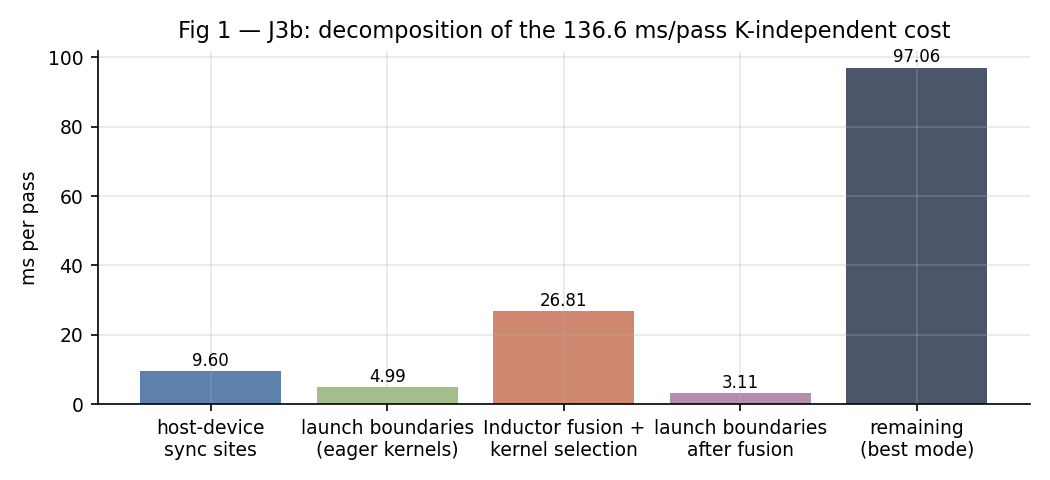
\includegraphics[width=.85\textwidth]{figures/fig1_j3b_decomposition.png}
\caption{Part A. Decomposition of the K-independent pass cost: sync sites, Inductor fusion, launch boundaries after fusion.}\label{fig:a1}\end{figure}
\begin{figure}[htbp]\centering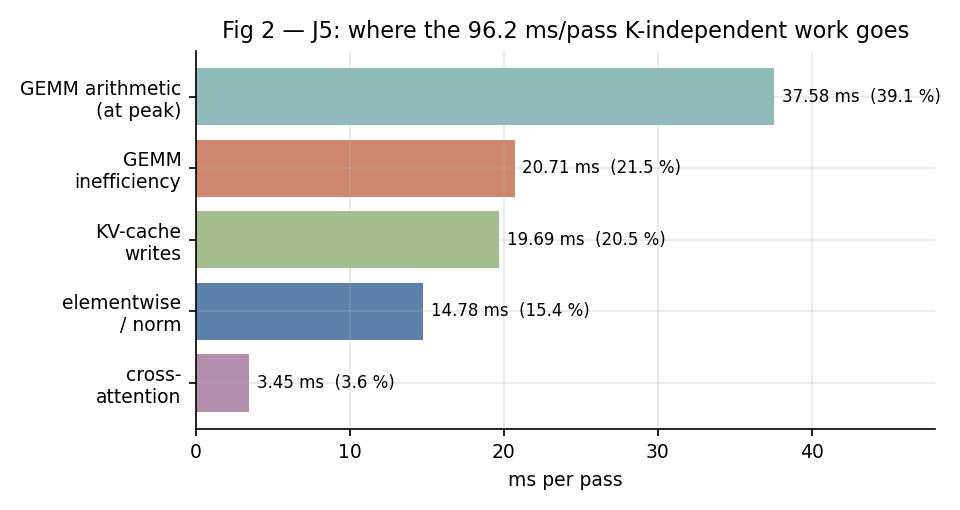
\includegraphics[width=.8\textwidth]{figures/fig2_j5_census.png}
\caption{Part A. Kernel census: where the K-independent work goes; only 39\% is tensor-core arithmetic at peak.}\label{fig:a2}\end{figure}
\begin{figure}[htbp]\centering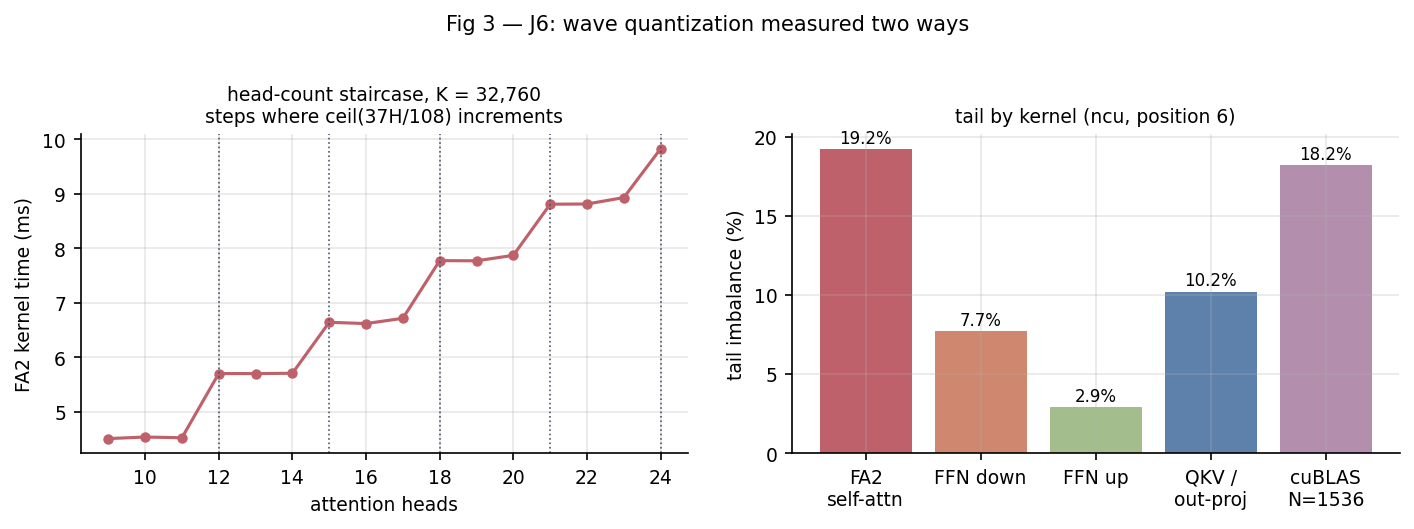
\includegraphics[width=\textwidth]{figures/fig3_j6_tails.png}
\caption{Part A. The FA2 wave-quantization tail measured by \texttt{ncu} and by the head-count staircase.}\label{fig:a3}\end{figure}
\begin{figure}[htbp]\centering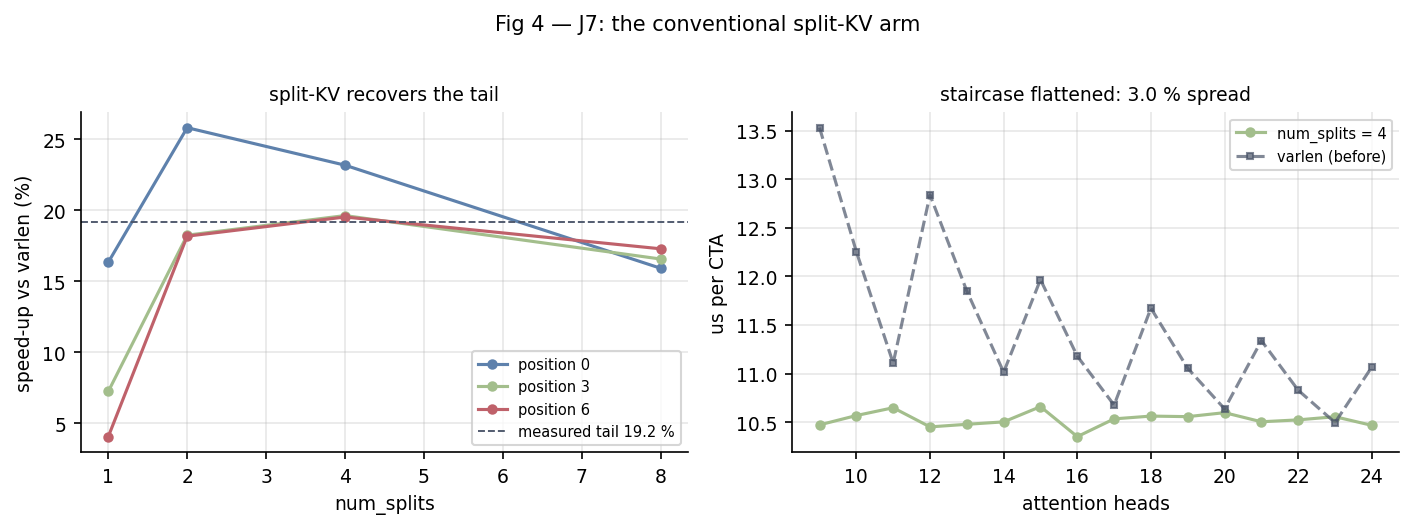
\includegraphics[width=\textwidth]{figures/fig4_j7_splitkv.png}
\caption{Part A. The split-KV arm and the flattened staircase; the FA2 heuristic alone recovers 3\%.}\label{fig:a4}\end{figure}
\begin{figure}[htbp]\centering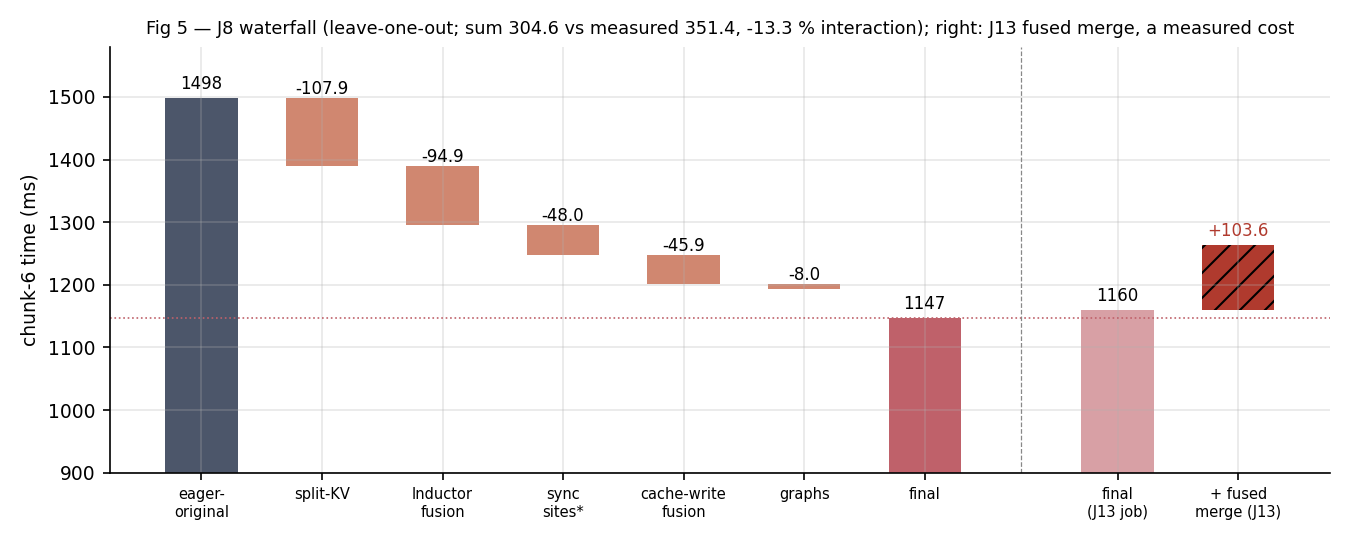
\includegraphics[width=\textwidth]{figures/fig5_j8_waterfall.png}
\caption{Part A. Waterfall from eager-original to \emph{final}; right, the J13 fused merge measured against its own \emph{final}: +103.7\,ms at chunk 6.}\label{fig:a5}\end{figure}
\begin{figure}[htbp]\centering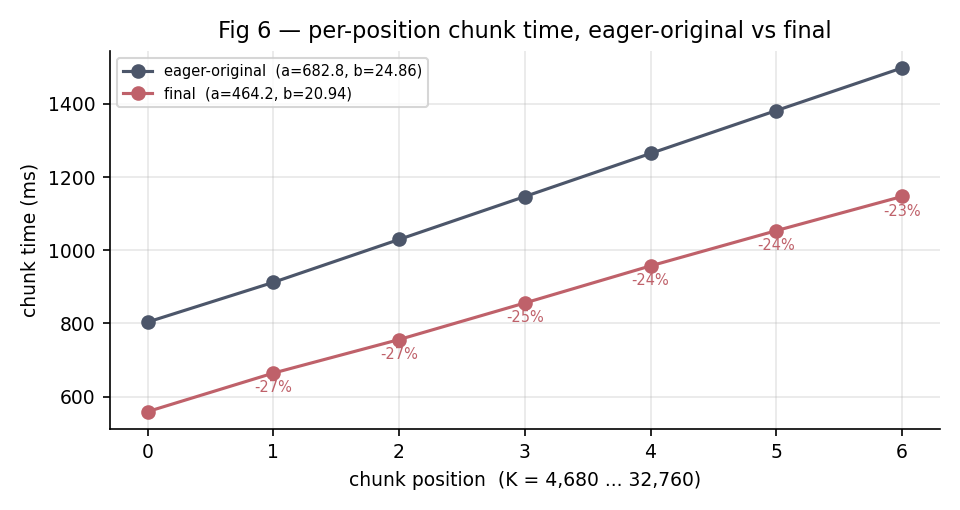
\includegraphics[width=.8\textwidth]{figures/fig6_per_position.png}
\caption{Part A. Per-position chunk time, eager-original versus \emph{final}.}\label{fig:a6}\end{figure}
\begin{figure}[htbp]\centering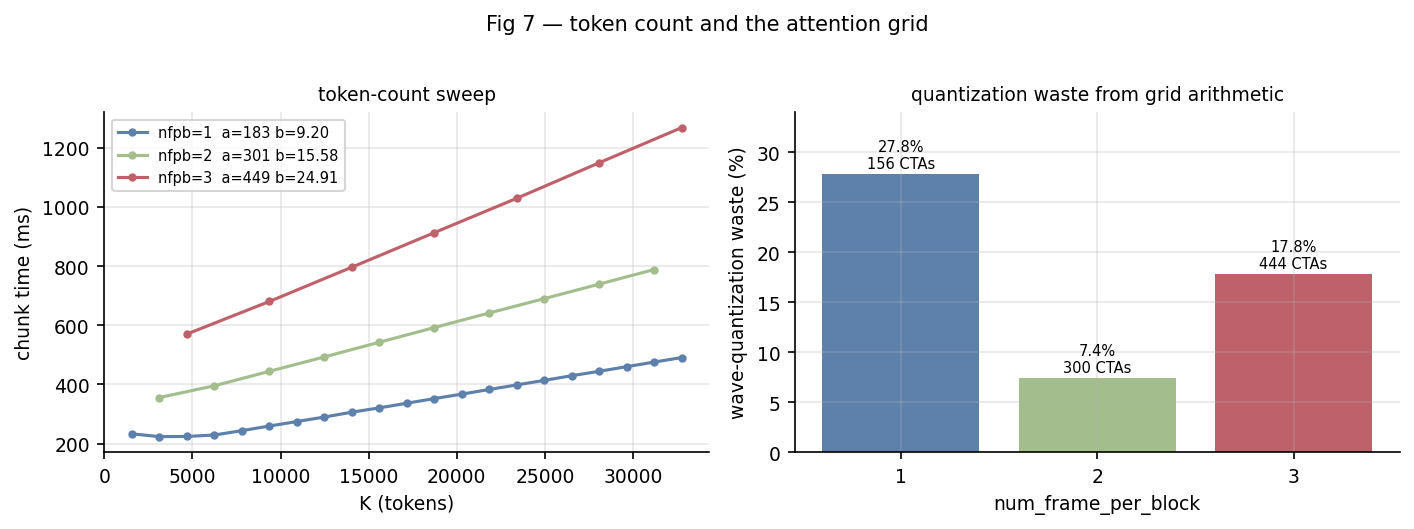
\includegraphics[width=\textwidth]{figures/fig7_nfpb_sweep.png}
\caption{Part A. Token-count sweep and the attention grid; the frame-level regime has the largest quantization waste by grid arithmetic.}\label{fig:a7}\end{figure}
\begin{figure}[htbp]\centering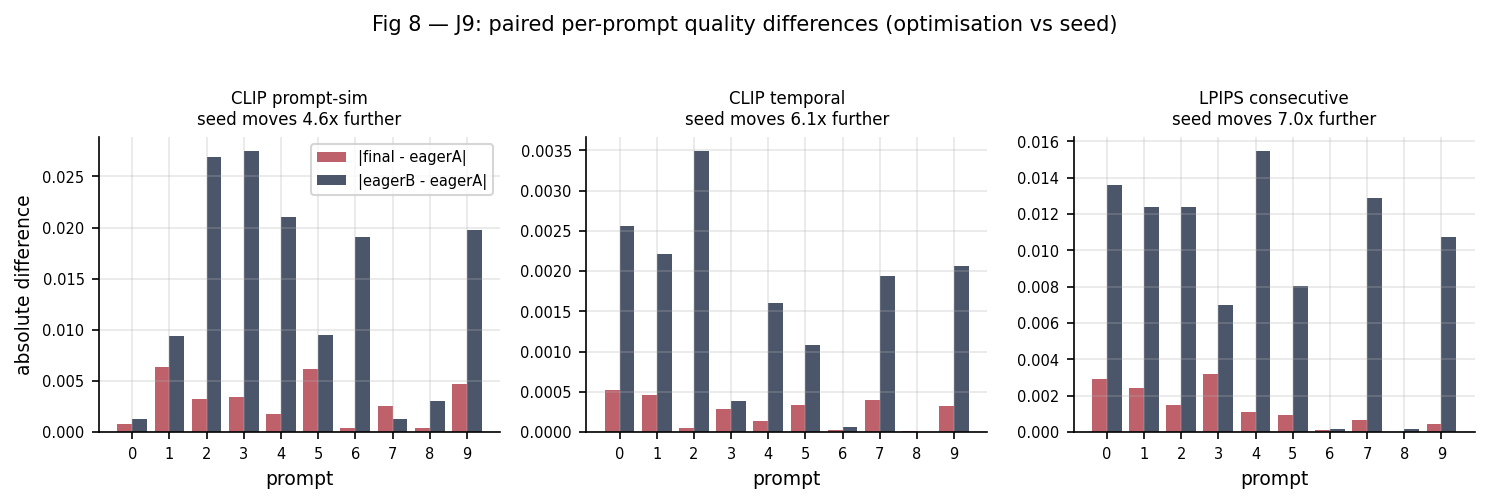
\includegraphics[width=\textwidth]{figures/fig8_j9_paired.png}
\caption{Part A. Paired per-prompt quality differences, \emph{final} versus eager-original, against a seed-to-seed control.}\label{fig:a8}\end{figure}
\begin{figure}[htbp]\centering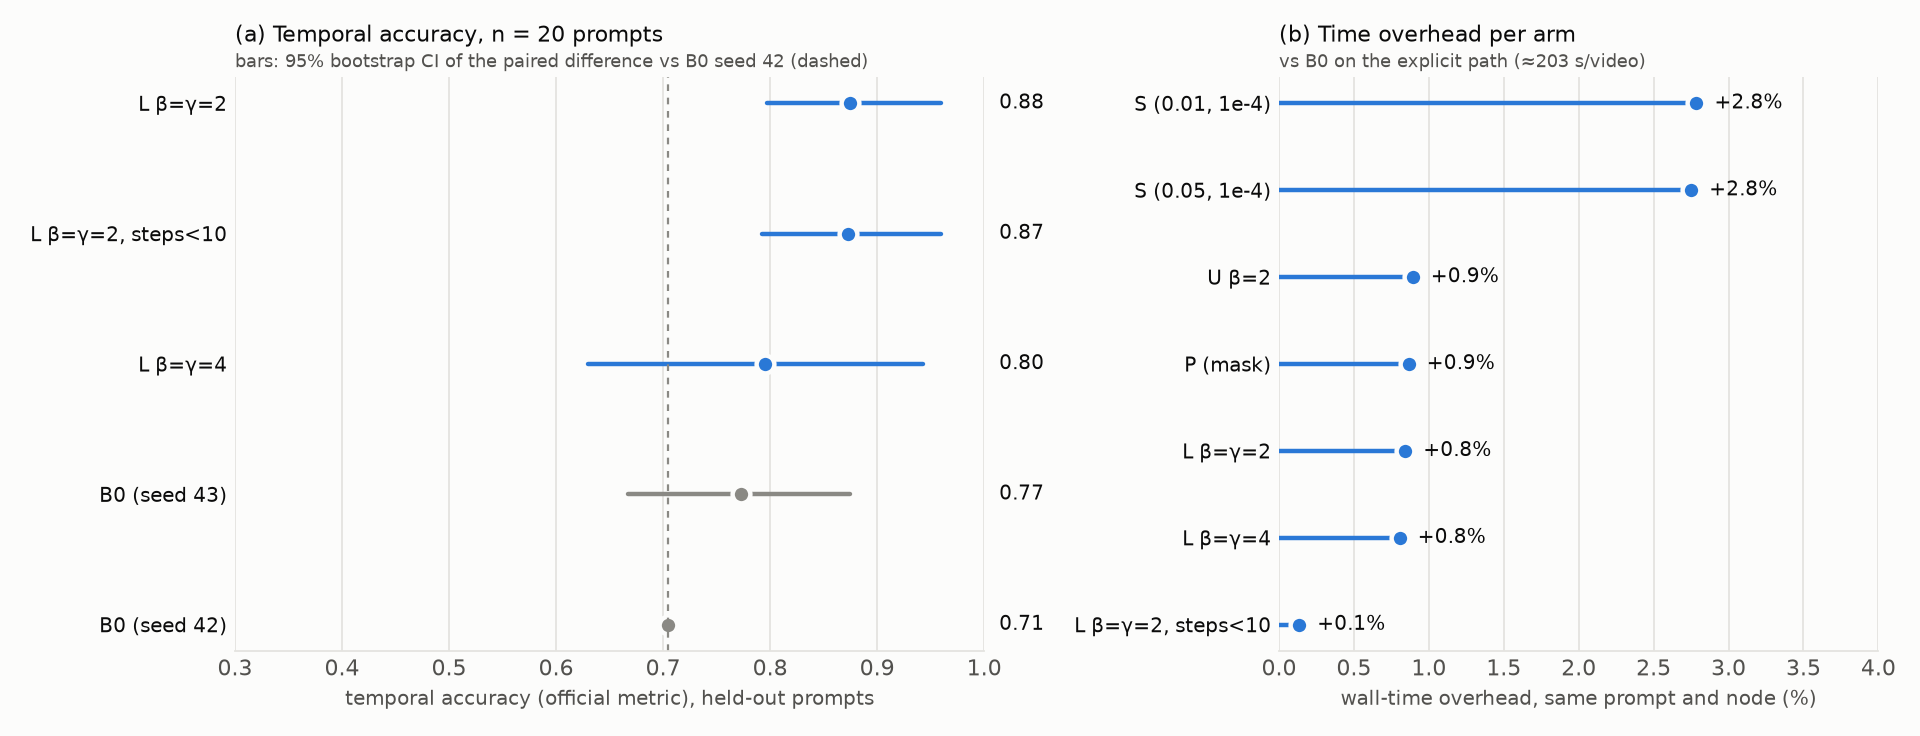
\includegraphics[width=\textwidth]{figures/findings_figure.png}
\caption{Part B. (a) Held-out temporal accuracy, 20 prompts, seed 42; dot = mean, bar = 95\% bootstrap CI of the paired difference against \arm{B0} seed 42 (dashed), centred on the run's mean; \arm{B0} seed 43 is the seed control. (b) Wall-time overhead per arm.}\label{fig:b1}\end{figure}
\begin{figure}[htbp]\centering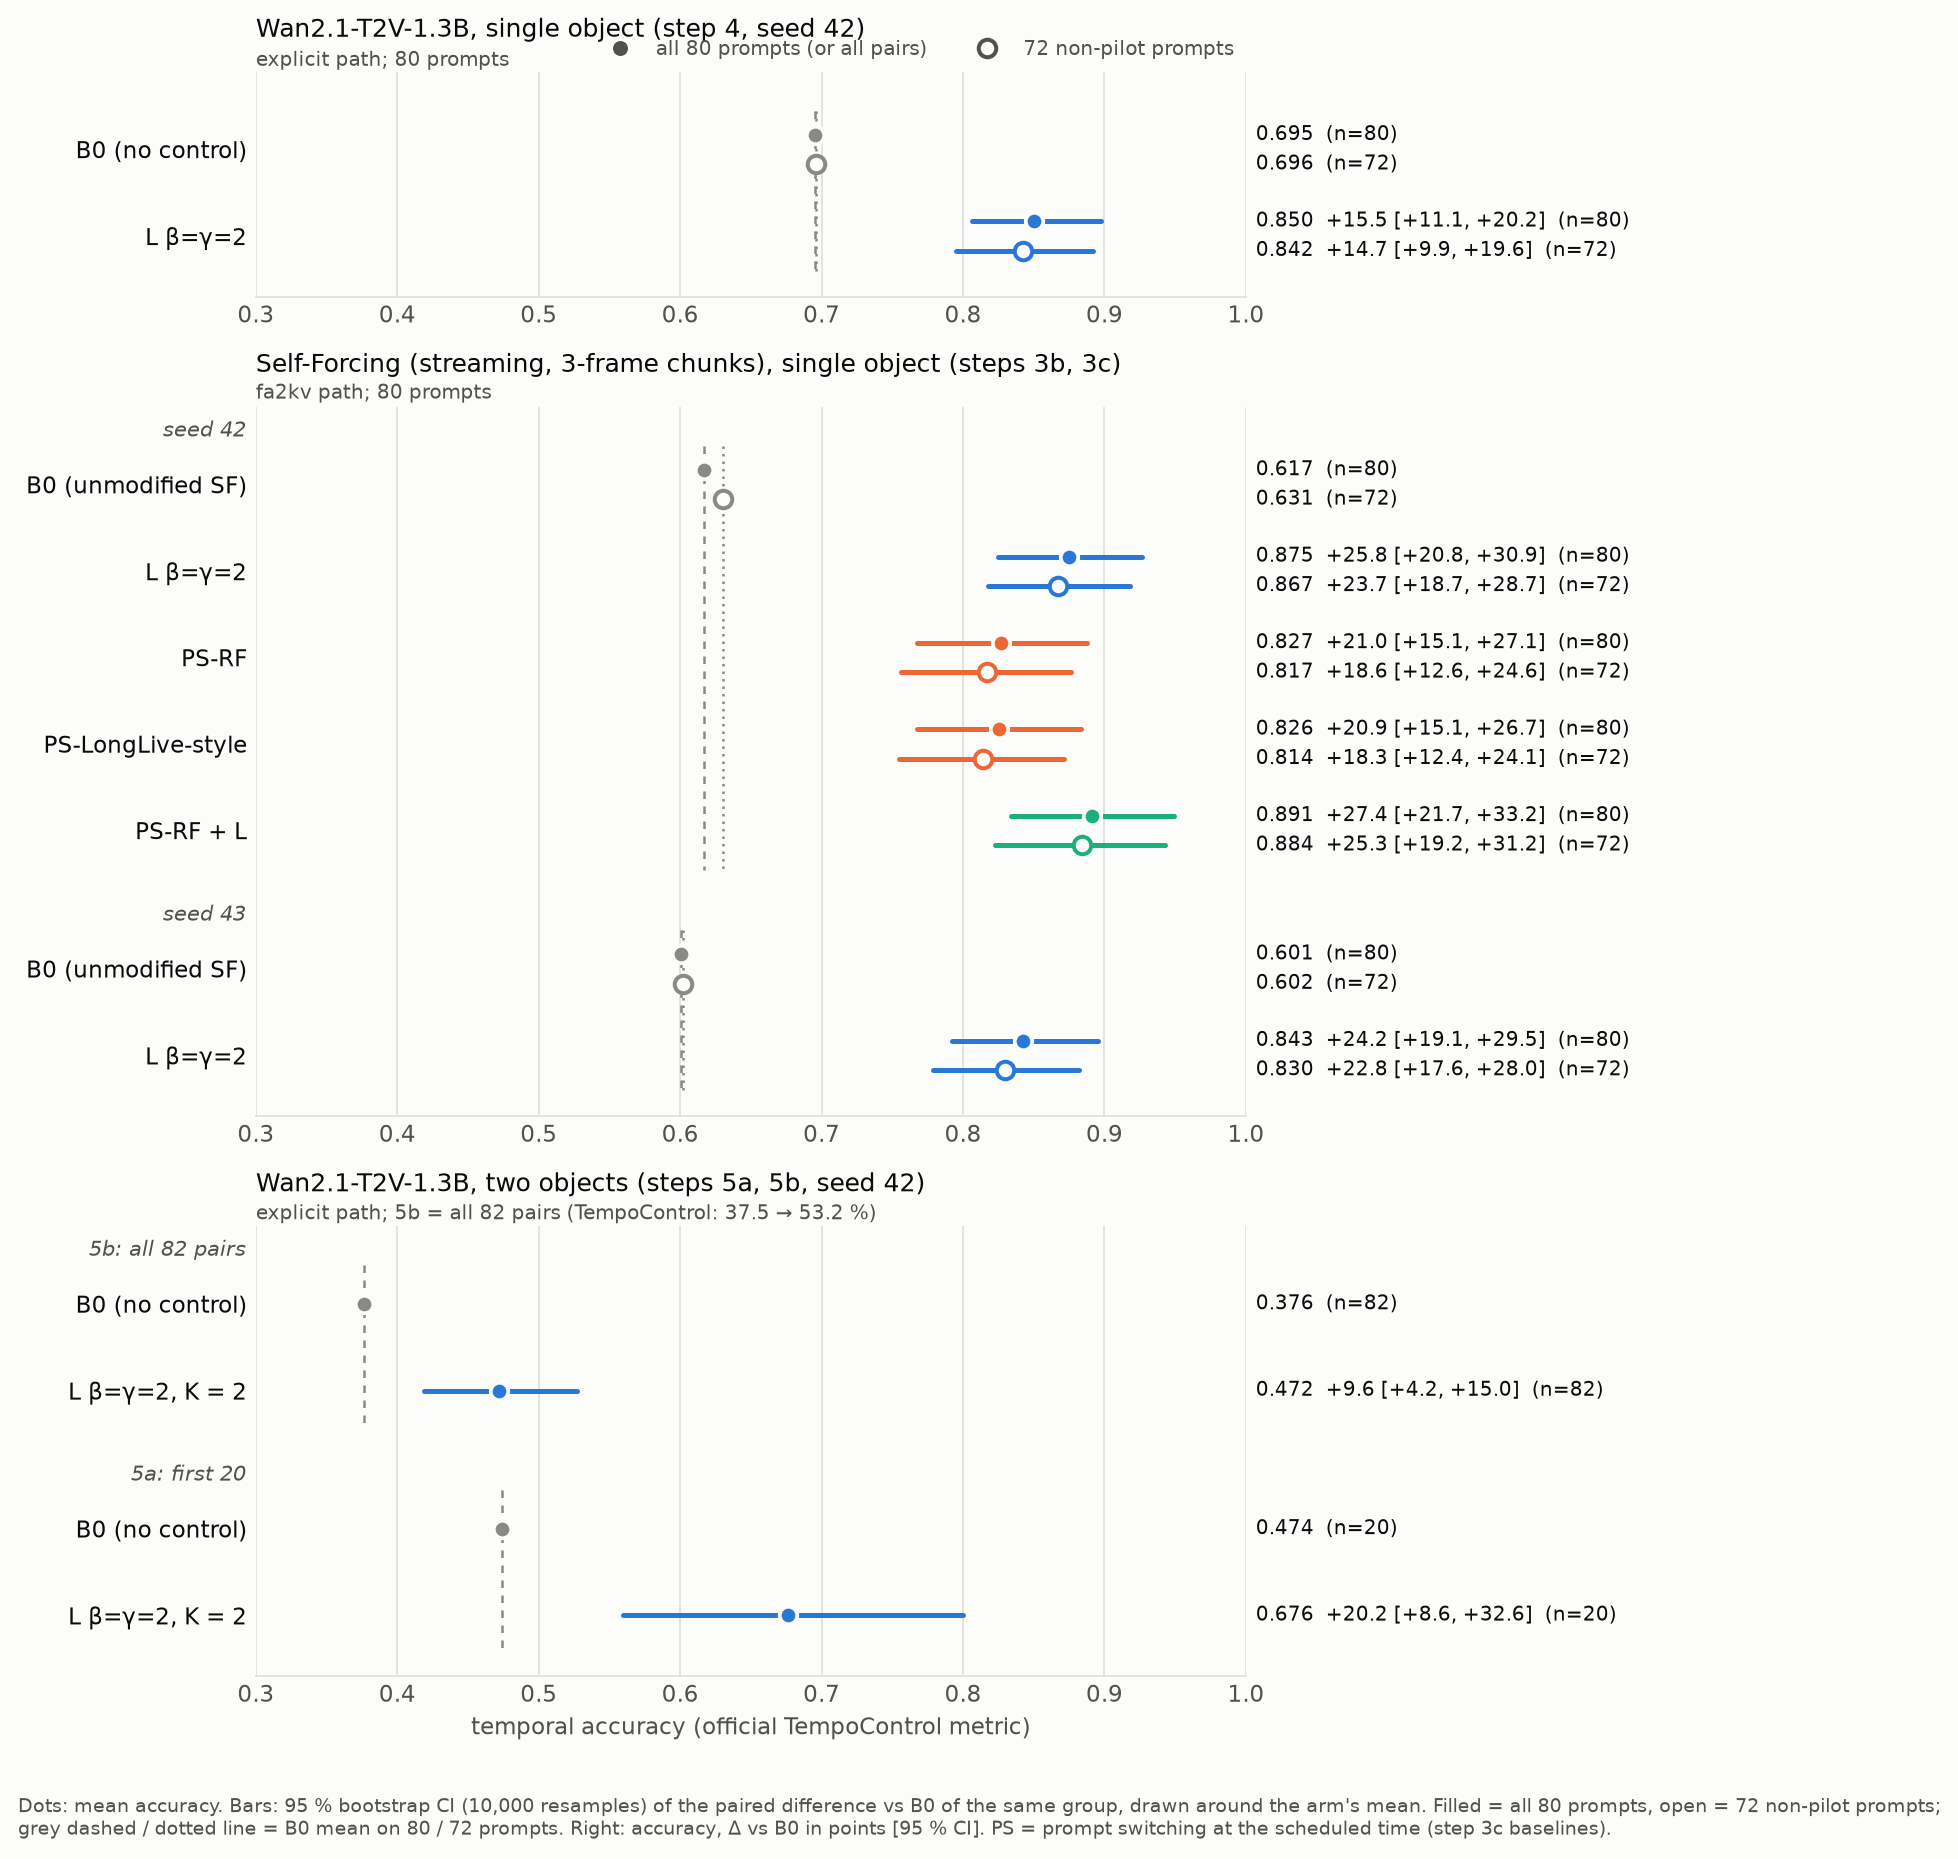
\includegraphics[width=.78\textwidth]{figures/fig_accuracy.png}
\caption{Part B. Accuracy per arm with 95\% CIs of the paired difference: Wan2.1 single object (80 prompts), Self-Forcing single object (80 prompts, two seeds, with prompt-switching baselines), Wan2.1 two objects (82 pairs).}\label{fig:b2}\end{figure}
\begin{figure}[htbp]\centering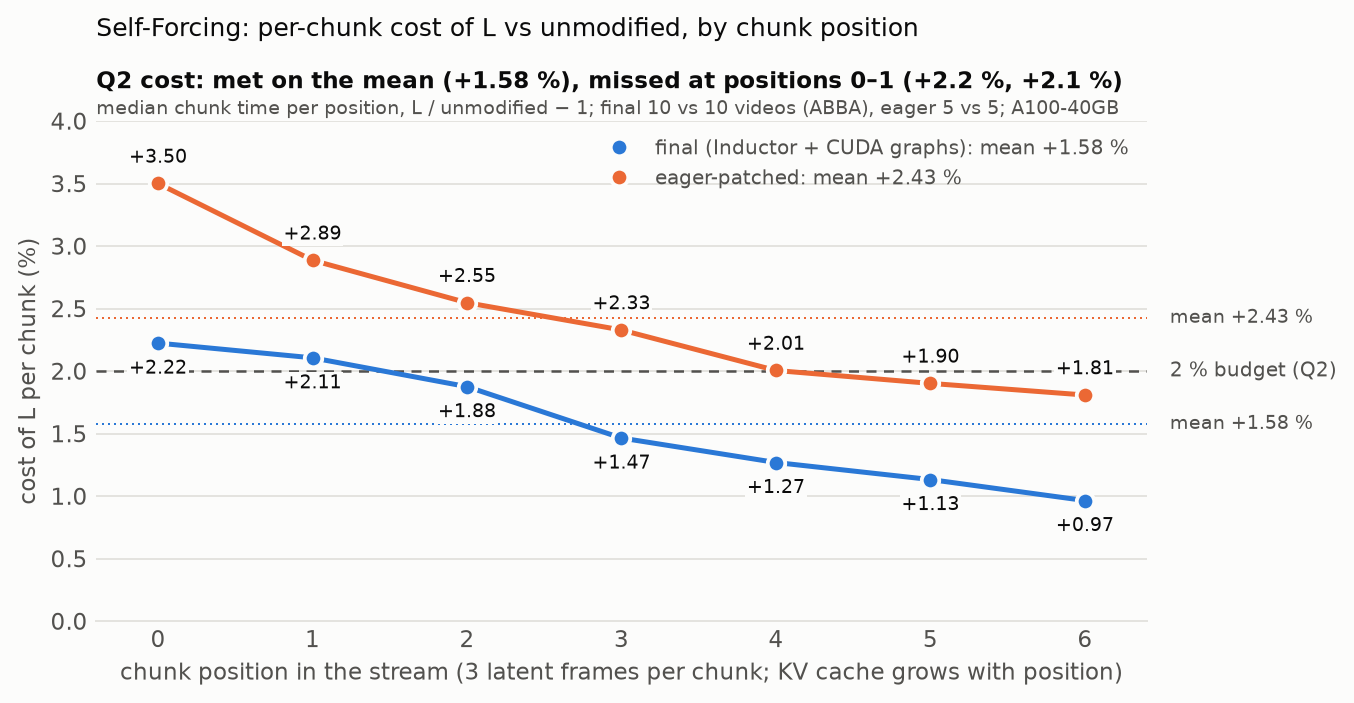
\includegraphics[width=.9\textwidth]{figures/fig_sf_block_cost.png}
\caption{Part B. Per-chunk cost of \arm{L} inside Self-Forcing in Part A's latency protocol.}\label{fig:b3}\end{figure}
\begin{figure}[htbp]\centering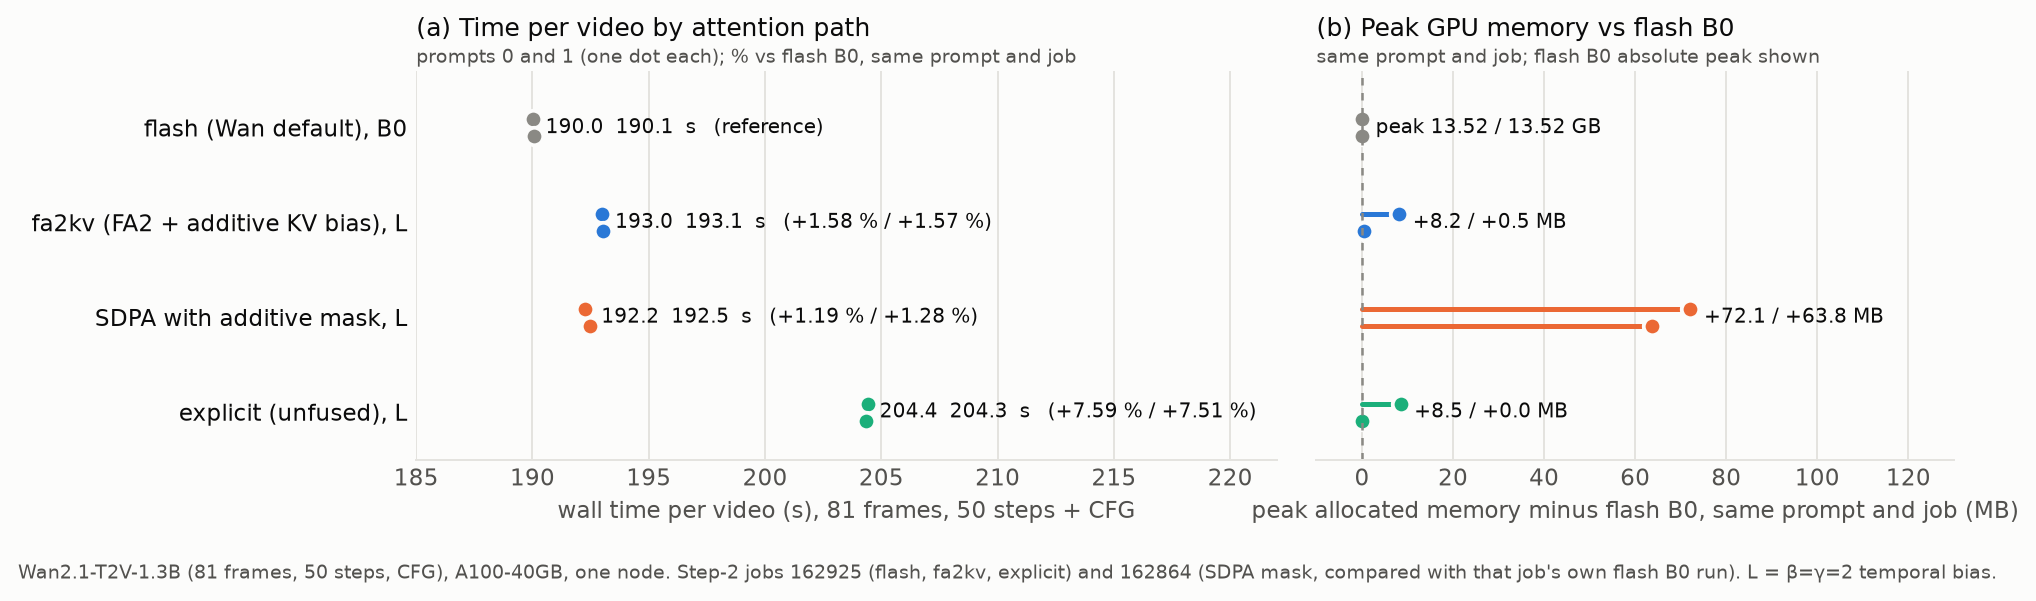
\includegraphics[width=\textwidth]{figures/fig_time_memory.png}
\caption{Part B. Time and memory per attention path: Wan's flash path, the explicit path, and fa2kv with \arm{L}.}\label{fig:b4}\end{figure}

\clearpage
\section*{Appendix A. Pre-registered predictions versus measurements}
\small
\textbf{Part A.} Every pre-registered prediction with its verdict; outcomes outside a band are MISS; no threshold was adjusted after a result was seen. Rows marked $\dagger$ are snapshot-verified (specification modification time earlier than the job's submit time). Rows labelled ``proposal'' are predictions from the project proposal; ``J6 (spec \S13)'' refers to section 13 of the J6 specification. nfpb = latent frames per chunk (3 in production, 1 in Fig.~\ref{fig:a7}); compile\_nocg = Inductor-compiled without CUDA graphs; eager-patched = eager-original with the sync sites removed.

\begin{tabularx}{\textwidth}{lYYl}\toprule
job & prediction & measured & verdict\\\midrule
proposal & coordination after graphs 8-15\% of chunk & launch-boundary component $\approx1\%$; intra-kernel tail 9.5-12.1\% & split\\
proposal & coordination fraction grows as tokens shrink & +22\% K-independent cost per token at nfpb=1 & HIT (proxy)\\
proposal & fusion recovers about half of elementwise cost & fusion 26.8\,ms/pass; elementwise cost before fusion not measured & not measurable\\
J2 & chunk-6 spread $<3\%$ & 0.106\% & HIT\\
J3 & PSNR floor $>40$\,dB & 14.4\,dB; metric retired & MISS\\
J5 & N=1536 GEMMs at 55-70\% peak & 53.9, 57.9, 59.0, 59.9\% & 3 of 4 (partial MISS)\\
J5 & N$\ge$4608 GEMMs at 75-85\% peak & 63.1\% and 74.4\% & MISS\\
J5 & elementwise+norm $\ge10$\,ms/pass & 14.78 & HIT\\
J5 & cross-attention $\ge5$\,ms/pass & 3.45 & MISS\\
J5 & N=1536 GEMMs at 4.1 waves with visible last-wave quantization & 2.06 waves; quantization severe (6\% last wave) & half-HIT\\
J6 & FFN down tail $\ge25\%$ & 7.7\% & MISS\\
J6 & FFN up and QKV tails $<8\%$ & 2.9\% and 10.2\% & split\\
J6 & FA2 tail $<5\%$ & 19.2\% & MISS (opposite)\\
J6 & inter-kernel gaps $\le1.5\%$ of pass & 0.57\% (traced in compile\_nocg; an upper bound) & HIT (mode deviation)\\
J6c & $\ge15$ of 19.7\,ms/pass cache-write recovered & 10.71 (54\%) & MISS\\
J7$\dagger$ & slope $b$ falls 12-16\% & 16.98\% & MISS (high side)\\
J7$\dagger$ & intercept unchanged & +6.25\% (combine cost) & MISS\\
J8 & intercept ratio 0.62-0.66 & 0.6799 & MISS\\
J8 & slope ratio $\approx0.83$ & 0.8421 & HIT\\
J8 & chunk-6 1050-1100\,ms & 1147.0 & MISS\\
J8 & waterfall order split-KV $>$ Inductor $>$ cache-write $>$ sync $>$ graphs & split-KV $>$ Inductor $>$ sync (48.0) $>$ cache-write (45.9) $>$ graphs & MISS on ranks 3/4\\
J6 (spec \S13) & FA2 staircase steps at H=6,12,18,24; per-CTA cost constant within a step & steps at H=12,15,18,21,24 (wave = 108 CTAs); per-CTA cost declines within a step & MISS\\
J13 A1$\dagger$ & fused merge recovers 3-5\,ms/pass; intercept $-15$..$-25$\,ms/chunk; slope within 1\% & +20.05\,ms/pass; slope +0.44\% & MISS (slope HIT)\\
J13 A2$\dagger$ & chunk 0 faster than eager-patched with split-KV, crossover gone; chunk 6 $-1.3$..$-2.2\%$ & chunk 0 +18.0\%, chunk 6 +8.9\% & MISS\\
J13 A3$\dagger$ & fused tensor-pipe utilisation within 10\% of the unfused GEMM & 9.0\% vs 80.7\% & MISS\\
J13 A4$\dagger$ & fp32-band agreement at every position & ratio 1.00 at 14/14; in situ identical to final & HIT\\
J13 B$\dagger$ & negative result, $-1$..$+1.5$\,ms/pass, L2-bound & +20\,ms/pass (slower); register/occupancy-bound with spills & direction HIT, size and mechanism MISS\\
\bottomrule\end{tabularx}

\medskip
\textbf{Part B.} Every prediction was committed to the experiment specification with its date and git commit before the run it concerns. Ids: P1-P6 are the Phase 1/2 predictions; Q1-Q6 the gates of the fused path, streaming cost, calibration, full benchmark, two objects and VBench; P3b-1/2 the streaming and prompt-switching predictions; PA and PB the later-added predictions for the fa2kv accuracy check and the 82-pair run; ``step 2'' and ``3c'' are the correctness test and the machinery gates of those steps. SDPA mask = the first fused-path candidate, an additive mask passed to PyTorch's scaled-dot-product attention.

\begin{tabularx}{\textwidth}{lYYl}\toprule
id & prediction & measured & verdict\\\midrule
P1 & \arm{U} does not raise accuracy beyond the seed spread & +0.012 [$-0.056$, +0.081], 3/3 & Met\\
P2 & best of \arm{L}/\arm{S}/\arm{P} gains $\ge+10$ points over \arm{B0} & \arm{L}(2,2): +17.0 (s42), +12.3 (s43), +14.6 pooled & Met\\
P3 & \arm{S} matches or beats \arm{L} & \arm{S} 0.59 vs \arm{L} 0.92 on the pilot; \arm{S} erases the object & Missed\\
P4 & best arm overhead $\le10\%$; memory change $\le1$\,GB & +0.8\%; memory unchanged & Met\\
P5 & editing only steps $<10$ keeps $\ge80\%$ of the gain & 99\% (s42), 67\% (s43), 85\% pooled & Mixed\\
P6 & CLIP change within the seed spread & $-0.013$ [$-0.019$, $-0.007$]; spread sd 0.024 & Met as worded; consistent drop\\
Q1 & fa2kv \arm{L} within 2\% of flash time; memory $\pm0.5$\,GB & +1.58\%, +0.008\,GB & Met\\
step 2 & fused output $\le$ flash's error vs fp64 at 9 probes & missed by SDPA mask and by fa2kv-L; replacement criterion defined after & Missed\\
Q2 & Self-Forcing: \arm{L} $\le2\%$ block time and raises accuracy & accuracy met (+25.8/+24.2); cost +1.58\% mean, +2.2\%/+2.1\% at positions 0-1 & Met / mixed\\
P3b-1 & Self-Forcing, 72 non-pilot: $\ge+12$ at s42, same sign at s43 & +23.7 / +22.8 & Met\\
P3b-2 & prompt switching: absent $\ge0.90$; $>$ \arm{B0}; switch $\le+5\%$ & 0.96; +17.5; +0.36\% & Met\\
Q3 & Wan \arm{B0} on all 80 within $\pm5$ of 63.9\% & 69.5\% & Missed\\
Q4 & Wan \arm{L} on 72 non-pilot $\ge+12$, CI excluding 0 & +14.7 [+9.9, +19.6] & Met\\
Q5 & two objects: \arm{L} $\ge+8$ on 20 scorable pairs & +20.2 [+8.6, +32.6] & Met\\
PA & fa2kv \arm{L} $-$ flash \arm{B0} $>0$ on 20 held-out & +17.2 [+9.0, +26.7] & Met\\
PB & 5b: \arm{L} $-$ \arm{B0} $>0$ on all 82 pairs & +9.6 [+4.2, +15.0]; baselines agree & Met\\
Q6 & VBench $\Delta$ within the seed spread & imaging quality $-0.043$, CI excludes 0; subject consistency +0.004 & Missed / met\\
3c & machinery gates M0-M5 & all passed & - \\
\bottomrule\end{tabularx}

\section*{Appendix B. Budget and reproducibility}
\small
Part A ran thirteen jobs (J1-J13) on \texttt{a100-public}; every figure regenerates from \texttt{latency/results/*.json} without a GPU (\texttt{src/plotting/make\_figures.py}). Part B used 13.01 A100 GPU-hours for Part 1 (210 videos: Phase 0 1.11, pilot 3.77, held-out and replication 8.13) and 22.80 for Part 2 (steps 2-3b 3.01, full 80-prompt benchmark 6.00, prompt-switching baselines 1.20, two objects 2.48 + 7.40, VBench 0.19, production-path accuracy check with GPU-scoring gates 2.52); scoring on the GPU was shown to equal scoring on the CPU exactly (80/80 videos: 40 single-object and 40 two-object). Every video has one JSONL row (arm, parameters, prompt, seed, wall time, peak memory); every run configuration is in \texttt{tempo/runs/*.json} and every Slurm job in \texttt{tempo/slurm/}. Two independent audits recomputed every headline number of the final runs from the raw metric JSONs. Note on memory: the per-run peak-memory figures recorded by the generation script include the previous video's tensor; the audit of the final runs puts the clean peak at about 13.5\,GB rather than the 13.84\,GB recorded in every summary and quoted in this report.

\begin{thebibliography}{99}\small
\bibitem{selfforcing} X. Huang et al., ``Self Forcing: Bridging the Train-Test Gap in Autoregressive Video Diffusion,'' arXiv:2506.08009, 2025; code github.com/guandeh17/Self-Forcing, revision 33593df3.
\bibitem{wan} Wan Team, ``Wan: Open and Advanced Large-Scale Video Generative Models,'' arXiv:2503.20314, 2025; weights Wan-AI/Wan2.1-T2V-1.3B.
\bibitem{hazy} B. Spector et al. (Hazy Research), ``Look Ma, No Bubbles! Designing a Low-Latency Megakernel for Llama-1B,'' blog post, May 2025.
\bibitem{mpk} ``MPK: A Compiler and Runtime for Mega-Kernelizing Tensor Programs,'' arXiv:2512.22219; code github.com/mirage-project/mirage.
\bibitem{fa2} T. Dao, ``FlashAttention-2: Faster Attention with Better Parallelism and Work Partitioning,'' arXiv:2307.08691, 2023; flash-attn 2.8.3.
\bibitem{flashdecoding} T. Dao, D. Haziza, F. Massa, G. Sizov, ``Flash-Decoding for long-context inference,'' blog post, Oct 2023.
\bibitem{lean} R. Sanovar et al., ``Lean Attention: Hardware-Aware Scalable Attention Mechanism for the Decode-Phase of Transformers,'' arXiv:2405.10480, 2024.
\bibitem{tempocontrol} S. Schiber, O. Lindenbaum, I. Schwartz, ``TempoControl: Temporal Attention Guidance for Text-to-Video Models,'' arXiv:2510.02226, 2025. Code: github.com/Shira-Schiber/TempoControl (revision ac28c443, benchmark CSVs and \texttt{temporal\_accuracy.py} used unmodified); project page shira-schiber.github.io/TempoControl.
\bibitem{tsattn} H. Zhang, Y. Deng, Z. Pan, P.-T. Jiang, B. Li, Q. Hou, Z. Dou, Z. Dong, D. Zhou, ``TS-Attn: Temporal-wise Separable Attention for Multi-Event Video Generation,'' arXiv:2604.19473, 2026.
\bibitem{densediffusion} Y. Kim et al., ``Dense Text-to-Image Generation with Attention Modulation,'' arXiv:2308.12964, 2023.
\bibitem{promptrelay} G. Chen, Z. Huang, Z. Liu, ``Prompt Relay: Inference-Time Temporal Control for Multi-Event Video Generation,'' arXiv:2604.10030, 2026.
\bibitem{talc} H. Bansal et al., ``TALC: Time-Aligned Captions for Multi-Scene Text-to-Video Generation,'' arXiv:2405.04682, 2024.
\bibitem{peekaboo} Y. Jain et al., ``Peekaboo: Interactive Video Generation via Masked-Diffusion,'' arXiv:2312.07509, 2023.
\bibitem{longlive} S. Yang et al., ``LongLive: Real-time Interactive Long Video Generation,'' arXiv:2509.22622, 2025; code NVlabs/LongLive, v1 commit 9b2102b.
\bibitem{rollingforcing} K. Liu, W. Hu, J. Xu, Y. Shan, S. Lu, ``Rolling Forcing: Autoregressive Long Video Diffusion in Real Time,'' arXiv:2509.25161, 2025.
\bibitem{yolov10} A. Wang et al., ``YOLOv10: Real-Time End-to-End Object Detection,'' arXiv:2405.14458, 2024.
\bibitem{unipc} W. Zhao et al., ``UniPC: A Unified Predictor-Corrector Framework for Fast Sampling of Diffusion Models,'' arXiv:2302.04867, 2023.
\bibitem{vbench} Z. Huang et al., ``VBench: Comprehensive Benchmark Suite for Video Generative Models,'' arXiv:2311.17982, 2023; VBench 0.1.5.
\end{thebibliography}
\end{document}
